\documentclass[11pt, twoside, pdftex]{article}

% This include all the settings that we should use for the document
\newcommand{\PDFTitle}{Using GDB with Nios\textsuperscript{\textregistered} V}
\newcommand{\commonPath}{../../Common}
\newcommand{\datePublished}{Mar 2022}

\newcommand{\versnum}{21.1} %version number quartus/AMP
\newcommand{\quartusname}{Quartus\textsuperscript{\textregistered} Prime}	
\newcommand{\textBar}{For \quartusname{} \versnum{}}
\newcommand{\thisyear}{2022 } %for copyright
\newcommand{\company}{FPGAcademy.org}
\newcommand{\longteamname}{FPGAcademy.org}
\newcommand{\teamname}{FPGAcademy}
\newcommand{\website}{FPGAcademy.org}

\newcommand{\productAcronym}{AMP}
\newcommand{\productNameShort}{Monitor Program}

\newcommand{\productNameMedTM}{Monitor Program}
\newcommand{\productNameMed}{Monitor Program}

%\newcommand{\headerLogoFilePath}[1]{#1/FPGAcademy.png}



\setlength\topmargin{-0.25in}
\setlength\headheight{0in}
\setlength\headsep{0.35in}
\setlength\textheight{8.5in}
\setlength\textwidth{7in}
\setlength\oddsidemargin{-0.25in}
\setlength\evensidemargin{-0.25in}
\setlength\parindent{0.25in}
\setlength\parskip{0in} 

\pdfpagewidth 8.5in
\pdfpageheight 11in

% listings is a package that supports encapsulating source code in LaTeX conveniently

\usepackage{listings}
% add support for graphics
\usepackage{graphicx}
\usepackage[usenames, dvipsnames]{color}

\def\expandparam\lstinputlisting[#1]#2{\edef\tmp{\noexpand\lstinputlisting[#1]{#2}}\tmp}

\widowpenalty 10000
\clubpenalty 10000

%%%%%%%%%%%%%%%%%%%% Source Code Formatting %%%%%%%%%%%%%%%%%%%%
\definecolor{globalCommentColour}{rgb}{0.588,0.588,0.588}

%%%%%%%%%%%%%%%%%%%%%%%%%%%%%%%%%%%%%%%%%%%%%%%%%%%%
% Defining a NiosII ASM highlighter for lstlisting
\lstdefinelanguage[NiosII]{Assembler} {
 	morekeywords={add, addi, and, andhi, andi, beq, bge, bgeu, bgt, bgtu, ble,  bleu, blt, bltu, bne, br, break,% 
 	bret, call, callr, cmpeq, cmpeqi, cmpge, cmpgei, cmpgeu, cmpgeui, cmpgt, cmpgti, cmpgtu, cmpgtui, cmple,%
 	cmplei, cmpleu, cmpleui, cmplt, cmplti, cmpltu, cmpltui, cmpne, cmpnei, custom, div, divu, eret, flushd,%
 	flushda, flushi, flushp, initd, initda, initi, jmp, jmpi, ldb, ldbio, ldbu, ldbuio, ldh, ldhio, ldhu, ldhuio,%
 	ldw, ldwio, mov, movhi, movi, movia, movui, mul, muli, mulxss, mulxsu, mulxuu, nextpc, nop, nor, or, orhi, ori,%
 	rdctl, rdprs, ret, rol, roli, ror, sll, slli, sra, srai, srl, srli, stb, stbio, sth, sthio, stw, stwio,%
 	sub, subi, sync, trap, wrctl, wrtcl, wrprs, xor, xori, xorhi, xori},% 	
 	morekeywords=[2]{.abort, .ABORT, .align, .app-file, .ascii, .asciz, .balign, .byte, .comm, .data, .def,%
 	.desc, .dim, .double, .eject, .else, .end, .endef, .endif, .equ, .equiv, .err, .extern, .file, .fill, .float,%
 	.global, .globl, .hword, .ident, .if, .include, .int, .irp, .irpc, .lcomm, .lflags, .line, .linkonce, .ln,%
 	.list, .long, .macro, .mri, .nolist, .octa, .org, .p2align, .psize, .quad, .rept, .sbttl, .scl, .section,%
 	.set, .short, .single, .size, .sleb128, .skip, .space, .stadb, .stabn, .stabs, .string, .symver, .tag,%
 	.text, .title, .type, .val, .uleb128, .word},% 	
 	morekeywords=[3]{et, bt, gp, sp, fp, ea, sstatus, ra, pc, status, estatus, bstatus, ienable, ipending, cpuid,%
 	exception, pteaddr, tlbacc, tlbmisc, eccinj, badaddr, config, mpubase, mpuacc},% 	
 	sensitive=t,%
 	alsoletter=.,%
	morestring=[b]",%
 	morecomment=[s]{/*}{*/},%
 	morecomment=[l]\#,%
   }[keywords,comments,strings]
   
   %% NOTE: morekeywords=[2] are GNU directives.
   
   \definecolor{niosInstructionColour}{rgb}{0.000,0.608,0.000}
   \definecolor{niosDirectiveColour}{rgb}{0.000,0.000,0.902}
   \definecolor{niosSpecialRegColour}{rgb}{0.000,0.000,0.000}
   \definecolor{niosStringColour}{rgb}{0.808,0.482,0.000}
   
   %% NOTE: To make bold use: =\bfseries\color{<colour>}
   \lstdefinestyle{defaultNiosStyle} {
   language=[NiosII]{Assembler},
   stringstyle=\color{niosStringColour},
   keywordstyle=\color{niosInstructionColour},
   keywordstyle=[2]\color{niosDirectiveColour},
   keywordstyle=[3]\itshape\color{niosSpecialRegColour}
   }
%%%%%%%%%%%%%%%%%%%%%%%%%%%%%%%%%%%%%%%%%%%%%%%%%%%%

%%%%%%%%%%%%%%%%%%%%%%%%%%%%%%%%%%%%%%%%%%%%%%%%%%%%
% Defining a ArmA9 ASM highlighter for lstlisting
\lstdefinelanguage[ArmA9]{Assembler} {
 	morekeywords={ADC, ADD, ADDS, AND, ANDS, B, BAL, BEQ, BGE, BGT, BL, BLT, BIC, BKPT, BLX, BNE, BX, CDP, CLZ, CMN, CMP, EOR,%
 	EORS, LDC, LDM, LDR, LDRB, LDRBT, LDRH, LDRSB, LDRSH, LDRT, LSL, MCR, MLA, MOV, MOVW, MOVT, MRC, MRS, MSR, MUL, MVN, ORR, PLD,%
 	ROR, RSB, RSC, SBC, SMLAL, SMULL, STC, STM, STR, STRB, STRBT, STRH, STRT, SUB, SUBS, SWI, SWP, SWPB, TEQ, UMLAL,
 	PUSH, POP, MOVS, RORS, LSR},%
 	morekeywords=[2]{.abort, .ABORT, .align, .app-file, .ascii, .asciz, .balign, .byte, .comm, .data, .def,%
 	.desc, .dim, .double, .eject, .else, .end, .endef, .endif, .equ, .equiv, .err, .extern, .file, .fill, .float,%
 	.global, .globl, .hword, .ident, .if, .include, .int, .irp, .irpc, .lcomm, .lflags, .line, .linkonce, .ln,%
 	.list, .long, .macro, .mri, .nolist, .octa, .org, .p2align, .psize, .quad, .rept, .sbttl, .scl, .section,%
 	.set, .short, .single, .size, .sleb128, .skip, .space, .stadb, .stabn, .stabs, .string, .symver, .tag,%
 	.text, .title, .type, .val, .vectors, .uleb128, .word},%
 	morekeywords=[3]{SP, PC, MIDR, CTR, TCMTR, TLBTR, MPIDR, ID_PFR0, ID_PFR1, ID_DFR0, ID_MMFR0, ID_MMFR1, ID_MMFR2,%
 	ID_MMFR3, ID_ISAR0, ID_ISAR1, ID_ISAR2, ID_ISAR3, ID_ISAR4, CCSIDR, CLIDR, AIDR, CSSELR, TTBR0, TTRB1, TTBR2, DACR,%
 	DFSR, IFSR, ADFSR, AIFSR, DFAAR, IFAR, ICIALLUIS, BPIALLIS, PAR, ICIALLU, ICIMVAU, BPIALL, DCIMVAC, DCISW, V2PCWPR,%
 	DCCVAC, DCCSW, DDIMVAC, DCISW, TLBALLIS, TLBIMVAIS, TLBIASIDIS, TLBIMVAAIS, TLBIALL, TLBIMVA, TLBIASID, TLBIMVAA,%
 	PMCR, PMCNTENSET, PMCNTENCLR, PMOVSR, PMSWINC, PMSELR, PMXEVTYPER, PMXEVCNTR, PMUSERENR, PMINTENSET, PMINTENCLR,%
 	PRRR, NRRR, PLEIDR, PLEASR, PLEFSR, PLEUAR, PLEPCR, VBAR, MVBAR, ISR, FCSEIDR, CONTEXTIDR, TPIDRURW, TPIDRURO, TPIDRPRW},%
 	sensitive=f,%
 	alsoletter=.,%
	morestring=[b]",%
 	morecomment=[s]{/*}{*/},%
 	morecomment=[l]{//},%
   }[keywords,comments,strings]
   
   %% NOTE: morekeywords=[2] are GNU directives.
   
   \definecolor{armInstructionColour}{rgb}{0.000,0.608,0.000}
   \definecolor{armDirectiveColour}{rgb}{0.000,0.000,0.902}
   \definecolor{armSpecialRegColour}{rgb}{0.000,0.000,0.000}
   \definecolor{armStringColour}{rgb}{0.808,0.482,0.000}
   
   \lstdefinestyle{defaultArmStyle} {
   language=[ArmA9]{Assembler},
   stringstyle=\color{armStringColour},
   keywordstyle=\color{armInstructionColour},
   keywordstyle=[2]\color{armDirectiveColour},
   keywordstyle=[3]\itshape\color{armSpecialRegColour}
   }
%%%%%%%%%%%%%%%%%%%%%%%%%%%%%%%%%%%%%%%%%%%%%%%%%%%%

%%%%%%%%%%%%%%%%%%%%%%%%%%%%%%%%%%%%%%%%%%%%%%%%%%%%
% Defining style for the verilog.

\definecolor{verilogCommentColour}{rgb}{0.000,0.502,0.000}

\lstdefinestyle{defaultVerilogStyle} {
language={Verilog},
keywordstyle=\color{blue},
commentstyle=\color{verilogCommentColour}
}
%%%%%%%%%%%%%%%%%%%%%%%%%%%%%%%%%%%%%%%%%%%%%%%%%%%%

%%%%%%%%%%%%%%%%%%%%%%%%%%%%%%%%%%%%%%%%%%%%%%%%%%%%
% Defining style for the vhdl.
\lstdefinestyle{defaultVHDLStyle} {
language={VHDL},
keywordstyle=\color{blue},
commentstyle=\color{verilogCommentColour}
}
%%%%%%%%%%%%%%%%%%%%%%%%%%%%%%%%%%%%%%%%%%%%%%%%%%%%

%%%%%%%%%%%%%%%%%%%%%%%%%%%%%%%%%%%%%%%%%%%%%%%%%%%%
% Java
\definecolor{javaStringColour}{rgb}{0.808,0.482,0}
%%%%%%%%%%%%%%%%%%%%%%%%%%%%%%%%%%%%%%%%%%%%%%%%%%%%

%%%%%%%%%%%%%%%%%%%%%%%%%%%%%%%%%%%%%%%%%%%%%%%%%%%%
% Defining language styles
% C
\definecolor{CStringColour}{rgb}{0.808,0.482,0}
%%%%%%%%%%%%%%%%%%%%%%%%%%%%%%%%%%%%%%%%%%%%%%%%%%%%

%%%%%%%%%%%%%%%%%%%%%%%%%%%%%%%%%%%%%%%%%%%%%%%%%%%%
% Defining extended LaTeX language.
\lstdefinelanguage[LocalLaTeX]{TeX}[LaTeX]{TeX}%
 	{moretexcs={bf, it, sf, lstset},%
   	}%

\lstdefinestyle{defaultLocalLatexStyle} {
language=[LocalLatex]{TeX},
keywordstyle=\color{blue}\bfseries,
keywordstyle=[2]\color{blue},
keywordstyle=[3]\color{blue}\bfseries
}
%%%%%%%%%%%%%%%%%%%%%%%%%%%%%%%%%%%%%%%%%%%%%%%%%%%%

\lstset{
%language = C,
%language = Verilog,
%basicstyle=\color{black}\rmfamily\ttfamily,
basicstyle=\small\color{black}\ttfamily,
commentstyle=\small\color{globalCommentColour}\itshape\ttfamily,
keywordstyle=\small\color{blue}\bfseries\ttfamily,
showstringspaces=false,
frame=none, %lines % boxed listings
breaklines=true,
breakatwhitespace=true,
tabsize=4
}
%%%%%%%%%%%%%%%%%%%%%%%%%%%%%%%%%%%%%%%%%%%%%%%%%%%%%%%%%%%%%%%%


%\usepackage[centering]{geometry}.
%%%%%%%%%%%%%%%%%%%%%%%%%%%%%%%%%%%%%%%%%%%%%%%%%%%
% Document Settings
\usepackage[labelsep=period]{caption}
% we can choose a better font later
%\usepackage{palatino}
\usepackage{fourier}
%\fontencoding{T1}
% include common used symbols
\usepackage{textcomp}
% add support for graphics
\usepackage{graphicx}
\usepackage[usenames, dvipsnames]{color}
% enable to draw thick or thin table hlines
\setlength{\doublerulesep}{\arrayrulewidth}
\usepackage{longtable}
\setlongtables
%\usepackage{array}
% It may be better to use PDFLaTeX as it can generate bookmarks for the
% document

% Add some useful packages
\usepackage{ae,aecompl}
\usepackage{epsfig,float,times}

% reset the font for section
\usepackage{sectsty}
%\allsectionsfont{\fontfamily{ptm}\selectfont}
\allsectionsfont{\usefont{OT1}{phv}{bc}{n}\selectfont}

% use compact space for sections
\usepackage[compact]{titlesec}
\titlespacing{\section}{0pt}{0.2in}{*0}
\titlespacing{\subsection}{0pt}{0.1in}{*0}
\titlespacing{\subsubsection}{0pt}{0.05in}{*0}

% fancyhdr header and footer customization
\usepackage{layout}
\usepackage{fancyhdr}
\pagestyle{fancy}
\fancyhead{}
\fancyhead[R]{\textit{\tiny{\textBar}}}
\fancyfoot{}
\fancyfoot[LO,
RE]{\textrm{\href{https://www.fpgacademy.org}{\small \longteamname}} \\ {\small \datePublished }}
\fancyfoot[RO, LE]{\small \thepage}
% two-side settings
%\fancyhead{} % clear all header fields
%\fancyfoot{} % clear all footer fields
%\fancyfoot[LE,RO]{\thepage}
\renewcommand{\headrulewidth}{2pt}
\renewcommand{\headrule}{{\color{blue} \hrule width\headwidth height\headrulewidth \vskip-\headrulewidth}}
\renewcommand{\footrulewidth}{0pt}

% Format the footer on page 1
\fancypagestyle{plain}{
\fancyhead{}
\fancyfoot{}
\fancyfoot[LO,
RE]{\textrm{\href{https://www.fpgacademy.org}{\small \longteamname}} \\ {\small \datePublished }}
\fancyfoot[RO, LE]{\small \thepage}
\renewcommand{\headrulewidth}{0pt}
}
% adjust some setting to try to make the figure stay in the same page with text
% Reference: 	http://www.cs.uu.nl/~piet/floats/node1.html
%   			http://mintaka.sdsu.edu/GF/bibliog/latex/floats.html
%   General parameters, for ALL pages:
\renewcommand{\topfraction}{0.9}	% max fraction of floats at top
\renewcommand{\bottomfraction}{0.8}	% max fraction of floats at bottom
%   Parameters for TEXT pages (not float pages):
\setcounter{topnumber}{3}
\setcounter{bottomnumber}{3}
\setcounter{totalnumber}{5}     % 2 may work better
\setcounter{dbltopnumber}{2}    % for 2-column pages
\renewcommand{\dbltopfraction}{0.9}	% fit big float above 2-col. text
\renewcommand{\textfraction}{0.07}	% allow minimal text w. figs
%   Parameters for FLOAT pages (not text pages):
\renewcommand{\floatpagefraction}{0.7}	% require fuller float pages
% N.B.: floatpagefraction MUST be less than topfraction !!
\renewcommand{\dblfloatpagefraction}{0.7}	% require fuller float pages
%%%%%%%%%%%%%%%%%%%%%%%%%%%%%%%%%%%%%%%%%%%%%%%%%%%
% remember to use [htp] or [htpb] for placement
%%%%%%%%%%%%%%%%%%%%%%%%%%%%%%%%%%%%%%%%%%%%%%%%%%%

% set no indent for paragraph
\setlength{\parindent}{0em}
\addtolength{\parskip}{11pt}
\newcommand{\compact}{[topsep=0pt]}
% use this package to reduce space
\usepackage{enumitem}
\usepackage{multirow}
\usepackage{rotating}
\usepackage{pifont}
\usepackage{dingbat}
\newcommand{\itemsecond}{$\circ$}
%
%%%%%%%%%%%%%%%%%%
\date{}
\author{}
%%%%%%%%%%%%%%%%%%
\newcommand{\de}{DE-series}
\newcommand{\up}{FPGAcademy}
\newcommand{\fabric}{Avalon Switch Fabric}
\newcommand{\TODO}[1]{\textcolor{red}{\textbf{TODO}: #1}}
\def\registered{{\ooalign{\hfil\raise .00ex\hbox{\scriptsize R}\hfil\crcr\mathhexbox20D}}}

% enable url and reference(bookmarks) in pdf
\usepackage{url}
\usepackage[pdftex, colorlinks]{hyperref}
\hypersetup{%
pdftitle={\PDFTitle},
linkcolor=blue,
hyperindex=true,
pdfauthor={\longteamname},
pdfkeywords={FPGAcademy, Academic Program, Example System},
bookmarksnumbered,
bookmarksopen=false,
filecolor=blue,
pdfstartview={FitH},
urlcolor=blue,
plainpages=false,
pdfpagelabels=true,
linkbordercolor={1 1 1} %no color for link border
}%
%%%%%%%%%%%%%%%%%%%%%%%%%%%%%%%%%%%%%%%%%%%%%%%%%%%
\setlength{\fboxsep}{0.7pt}
\setlength{\fboxrule}{0.5pt}

\newcommand{\red}[1]{{\color{red}\sf{#1}}}
\newcommand{\blue}[1]{{\color{blue}\sf{#1}}}


\newcommand{\red}[1]{{\color{red}\sf{#1}}}

%%%%%%%%%%%%%%%%%%%%%%%%%
% Add title
\newcommand{\doctitle}{Using GDB with Nios\textsuperscript{\textregistered} V}
\newcommand{\dochead}{Using GDB with Nios\textsuperscript{\textregistered} V}
% Usually no need to change these two lines
\title{\fontfamily{phv}\selectfont{\doctitle} }
\chead{ \small{\textsc{\bfseries \dochead} } }
% Customizations
\newenvironment{ctabbing}%
{\begin{center}\begin{minipage}{\textwidth}\begin{tabbing}}
{\end{tabbing}\end{minipage}\end{center}}

%%%%%%%%%%%%%%%%%%%%%%%%%
% Allows multiple figures per page

\renewcommand\floatpagefraction{.9}
\renewcommand\topfraction{.9}
\renewcommand\bottomfraction{.9}
\renewcommand\textfraction{.1}   
\setcounter{totalnumber}{50}
\setcounter{topnumber}{50}
\setcounter{bottomnumber}{50}
\raggedbottom

%%%%%%%%%%%%%%%%%%
%%% DOCUMENT START
%\begin{document}
\begin{document}
\begin{table}
    \centering
    \begin{tabular}{p{5cm}p{4cm}}
        \hspace{-3cm}
        &
        \raisebox{1\height}{\parbox[h]{0.5\textwidth}{\Large\fontfamily{phv}\selectfont{\textsf{\doctitle}}}}
    \end{tabular}
    \label{tab:logo}
\end{table}

\colorbox[rgb]{0,0.384,0.816}{\parbox[h]{\textwidth}{\color{white}\textsf{\textit{\textBar}}}}

\thispagestyle{plain}
 
\section{Introduction}

This tutorial provides instructions for using the {\it GNU Project Debugger} (GDB) with the 
{\it Nios}\textsuperscript{\textregistered} {\it V} processor, to 
develop and debug software programs that are written in assembly-language or C code. 

This document is intended for a reader who is using a computer system with Nios~V on one of 
the DE-series boards that are described in the \texttt{Teaching and Projects Boards} 
section of the {\small \href{https://www.fpgacademy.org/boards.html} {FPGAcademy.org}} website.
We also assume that the reader is using a computer running a recent version of the 
{\it Windows}\textsuperscript{\textregistered} Operating system.

{\bf Required Software and Hardware}:
\begin{itemize}
\item Quartus Prime Programmer
\item GDB Server and Client for Nios~V
\item Nios~V computer system and DE-series FPGA board
\item Nios~V software development tools
\end{itemize}

{\bf Contents}:
\begin{itemize}
\item Installing the required software and hardware
\item Setting up the Nios~V development environment
\item Developing and debugging Nios~V assembly-language programs
\item Developing and debugging C programs
\item GDB command reference
\end{itemize}
\clearpage
\newpage

\section{Installing the Required Software and Hardware}
\label{sec:getthem}

The main software tools that are needed for this tutorial are the FPGA {\it Programmer
Tools} that accompany the Quartus Prime CAD system, the GDB server and client for Nios~V, and 
various Nios~V software development tools. The required hardware is a Nios~V computer
system that can be programmed into a DE-series FPGA board. The procedures for downloading and 
installing each of these components on your own computer are described below. A reader who 
is using a computer that already has the required software and hardware can skip ahead to 
Section~\ref{sec:setup}. 

\subsection{Installing the Quartus Prime Programmer Tools}
\label{sec:programmer}

The Nios~V processor is implemented as part of a computer system in an Altera FPGA device. 
In this tutorial we assume that the reader is using the {\it DE1-SoC Computer with Nios~V}.
A complete description of this system, describing all of the peripherals that are
connected to Nios~V, is available as part of the \texttt{Computer Organization} course 
on {\small \href{https://www.fpgacademy.org/courses.html} {FPGAcademy.org}}. If a
different computer system is being used, then some features of the hardware may not match
those described in this tutorial.

We assume that the user has access to a {\it DE1-SoC} board, and that this board has {\it not} 
already been programmed with the {\it DE1-SoC Computer with Nios~V}. Hence, programming of 
the board has to be performed, by using the {\it Quartus Prime Programmer} tools. This 
software can be obtained from the {\it Internet}, as discussed below. 

Three different Quartus Prime software {\it packages} are available, called {\it Pro},
{\it Standard}, and {\it Lite}. For each of these packages a number of {\it versions} are
released over time.  For any Quartus package, the {\it Programmer} tools can be 
obtained as a separate, {\it stand-alone}, program or as a part of a complete 
Quartus system. When used as a stand-alone program, the {\it Programmer} tools do not 
not require any license and are free to use. But if a complete Quartus Prime system 
were to be obtained and installed, then the {\it Pro} and {\it Standard} versions would 
require paid licenses, and only the {\it Lite} version could be used without a license. For 
this tutorial we use the {\it Programmer} as a stand-alone program. Perform the following
steps to download and install this program:

\begin{enumerate}
\item Search on the {\it Internet} for the \texttt{Intel (Altera) FPGA Software Download Center}. 
\item As illustrated in Figure~\ref{fig:down1}, select a \texttt{Software Package} and 
\texttt{Version}. For this tutorial we have selected \texttt{Quartus Prime Pro} and
\texttt{Version 24.1}.
\item Scroll down on the web page to see the types of \texttt{Downloads} that are
available. Click on the \texttt{Additional Software} category. Then, scroll further down 
on the web page to reveal the \texttt{Stand-Alone Software} programs. As illustrated in
Figure~\ref{fig:down2}, click on the button that is displayed to \texttt{Download} 
the \texttt{Quartus Prime Programmer and Tools}. You will need to accept an \texttt{Agreement},
after which a file will be downloaded to your computer.

The file downloaded above is an executable program (.{\it exe}).
Open the folder on your computer where this executable file has 
been downloaded and run the program. This action opens the installer dialogue depicted in 
Figure~\ref{fig:exe1}. Click \texttt{Next} to see the license agreement, which
must be accepted to install the software. Clicking \texttt{Next} again allows you to
select an installation folder. We recommend that you accept the default location which
should be similar to the one shown in Figure~\ref{fig:exe2}. Select \texttt{Next} to advance 
to the summary screen of the installation dialogue. On this screen you may see a message about 
obtaining a license to use the software, but {\bf do not} click on the provided link, because 
no license is required for the stand-alone {\it Programmer Tools}. Click \texttt{Next} on the
summary screen to install the {\it Programmer Tools}.

\begin{figure}[H]
    \begin{center}
        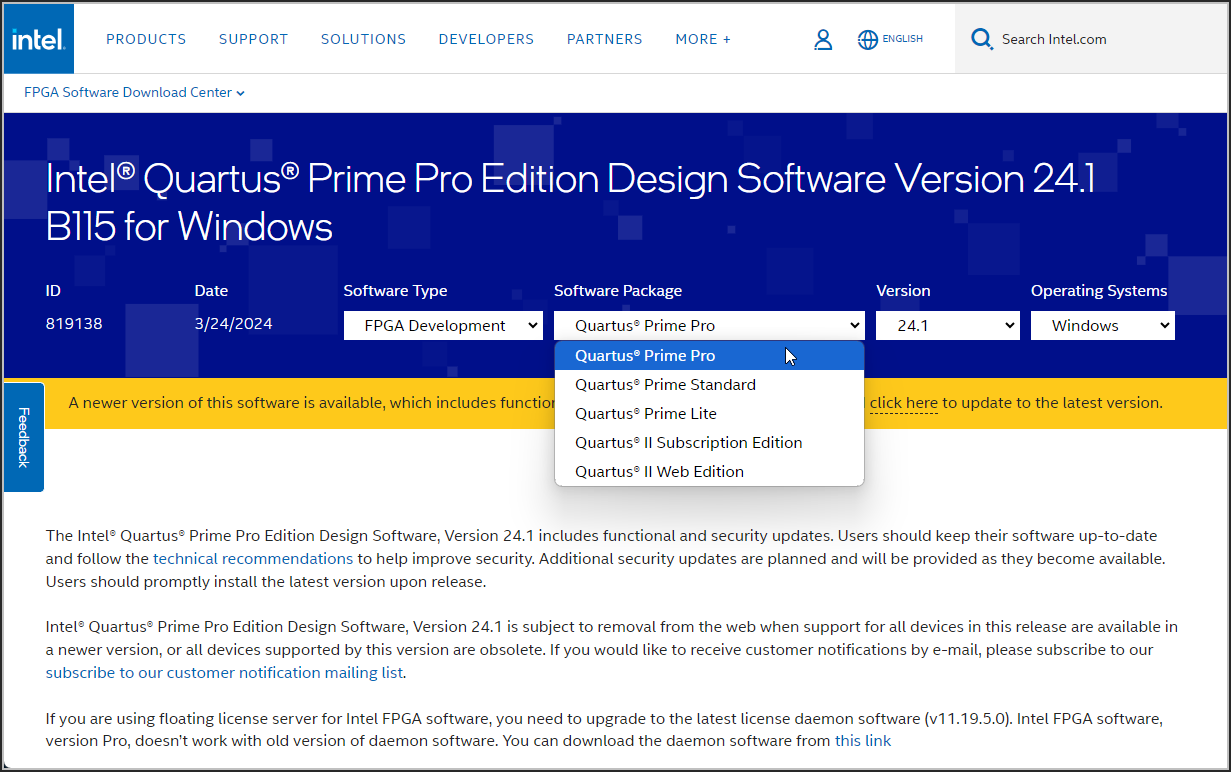
\includegraphics[width=.9\linewidth]{figures/down1.png}
        \caption{The Intel (Altera) FPGA Software Download Center.}
        \label{fig:down1}
    \end{center}
\end{figure}

\begin{figure}[H]
    \begin{center}
        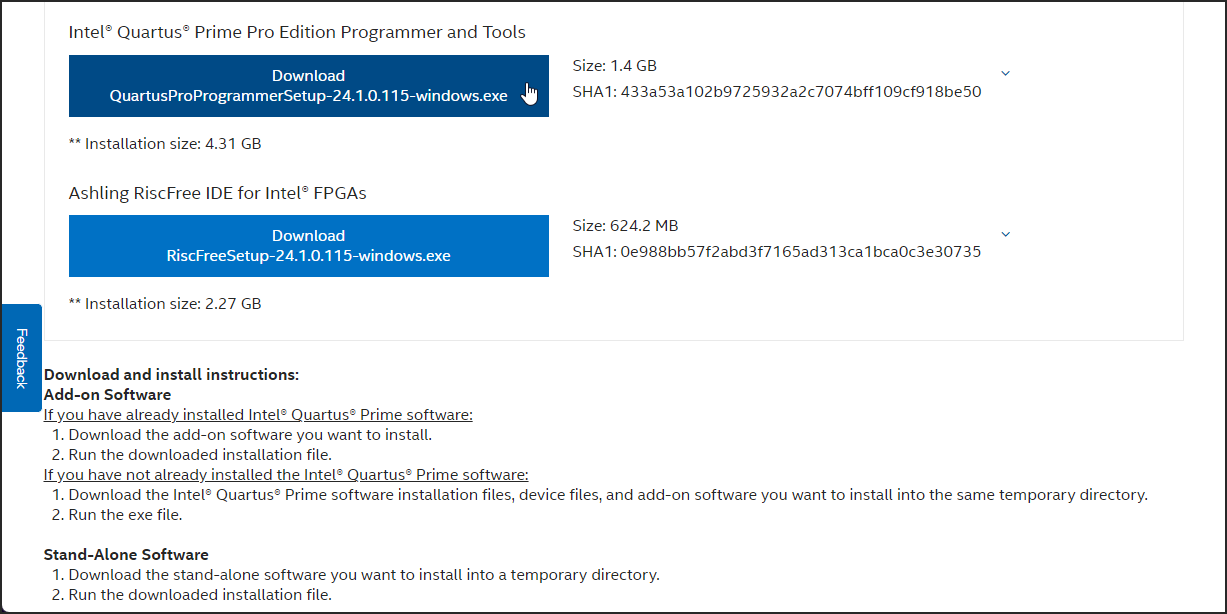
\includegraphics[width=.9\linewidth]{figures/down2.png}
        \caption{Downloading the Quartus Prime Programmer.}
        \label{fig:down2}
    \end{center}
\end{figure}

\begin{figure}[h]
    \begin{center}
        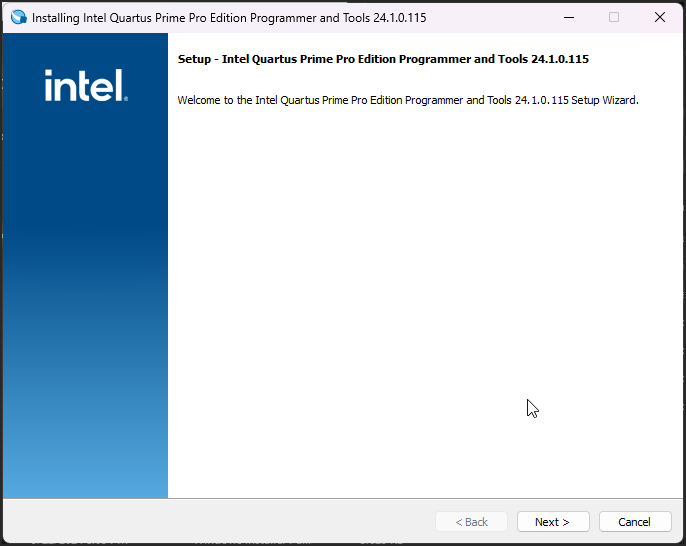
\includegraphics[scale=0.66]{figures/exe1.png}
        \caption{The {\it Programmer Tools} installation dialogue.}
        \label{fig:exe1}
    \end{center}
\end{figure}

\begin{figure}[h]
    \begin{center}
        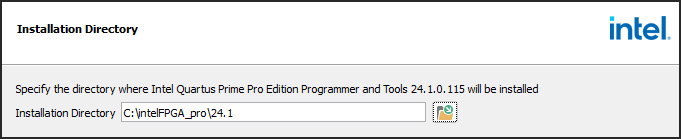
\includegraphics[scale=0.66]{figures/exe2.png}
        \caption{Choosing the installation folder.}
        \label{fig:exe2}
    \end{center}
\end{figure}

\begin{figure}[h]
    \begin{center}
        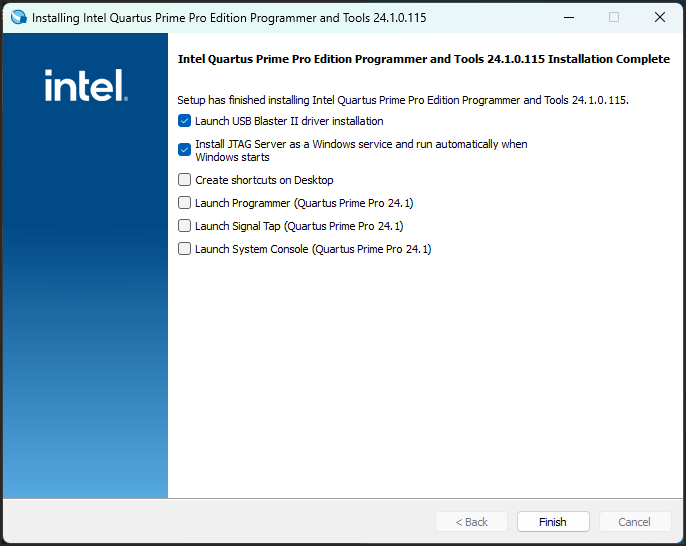
\includegraphics[scale=0.66]{figures/down2a.png}
        \caption{Post-installation selections.}
        \label{fig:down2a}
    \end{center}
\end{figure}

\item
After completing the {\it Programmer Tools} installation, the window displayed in 
Figure~\ref{fig:down2a} may appear. As the figure indicates you should make the
selections for installing the \texttt{USB Blaster II} driver and the \texttt{JTAG Server}. 
Click {\it Finish}. Depending on what device drivers are already installed on your computer 
you may be presented with additional installation dialogues. If so, follow the presented
steps to install the necessary drivers. These drivers allow for communication between your
computer and an FPGA board that is connected to the computer via a USB cable. 
\end{enumerate}

\newpage
\subsection{Installing the GDB Server and Client for Nios~V}
\label{sec:gdb}

The GDB software tools for Nios~V that are needed for this tutorial are available from the same 
\texttt{Intel (Altera) FPGA Software Download Center} used above to obtain the 
Quartus {\it Programmer Tools}. Navigate again to the website that is depicted in
Figure~\ref{fig:down1}. Again, scroll down on the website to see the types of
\texttt{Downloads} that are available, click on the \texttt{Additional Software} category,
and scroll further down to display the \texttt{Stand-Alone Software} programs. The 
GDB software tools for Nios~V are part of the package called 
\texttt{Ashling RiscFree IDE for Intel FPGAs}.
Click to download this package as indicated in Figure~\ref{fig:down3}, after which a file
will be downloaded to your computer.

The file downloaded above is an executable program (.{\it exe}).  Open the folder 
on your computer where this executable file has been downloaded and run the program.
This action opens the installer dialogue depicted in Figure~\ref{fig:exe3}. 
Click \texttt{Next} to see the license agreement, which
must be accepted to install the software. Clicking \texttt{Next} again allows you to
select an installation folder. This folder must be the {\it same} as the one that you
selected for the Quartus Programmer Tools, as mentioned previously for 
Figure~\ref{fig:exe2}. Select \texttt{Next} 
to advance to the summary screen of the installation dialogue. On this screen you may see a 
message about obtaining a license to use the software, but {\bf do not} click on the 
provided link, because no license is required for the this software package. After the
software has been installed, click \texttt{Finish} to close the installation executable.

\begin{figure}[H]
    \begin{center}
        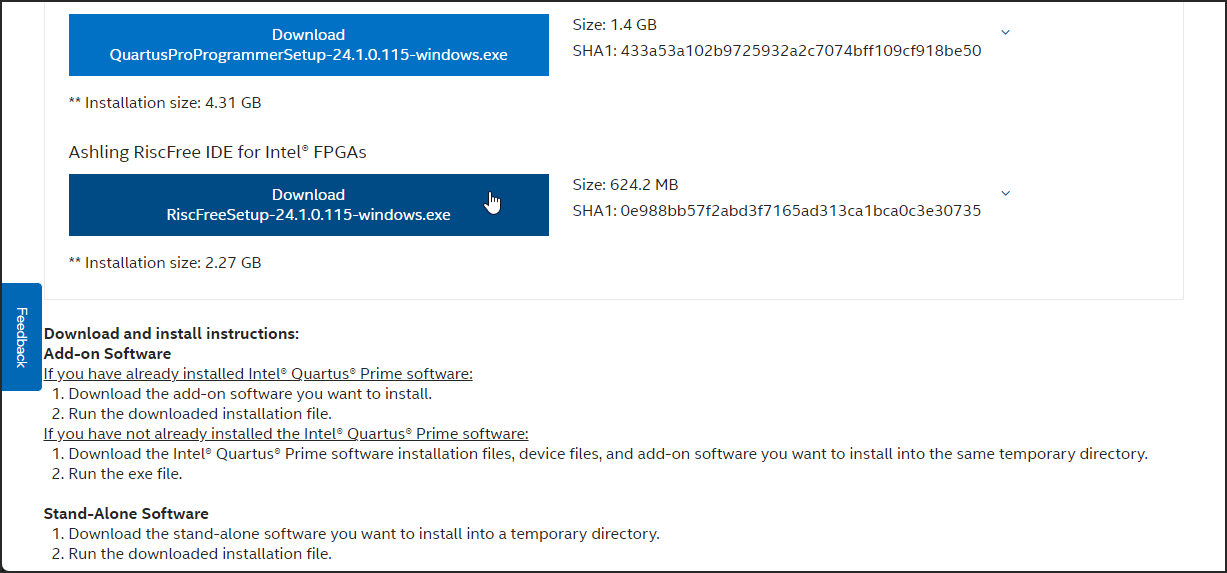
\includegraphics[width=.9\linewidth]{figures/down3.png}
        \caption{Downloading the GDB tools.}
        \label{fig:down3}
    \end{center}
\end{figure}

\begin{figure}[h]
    \begin{center}
        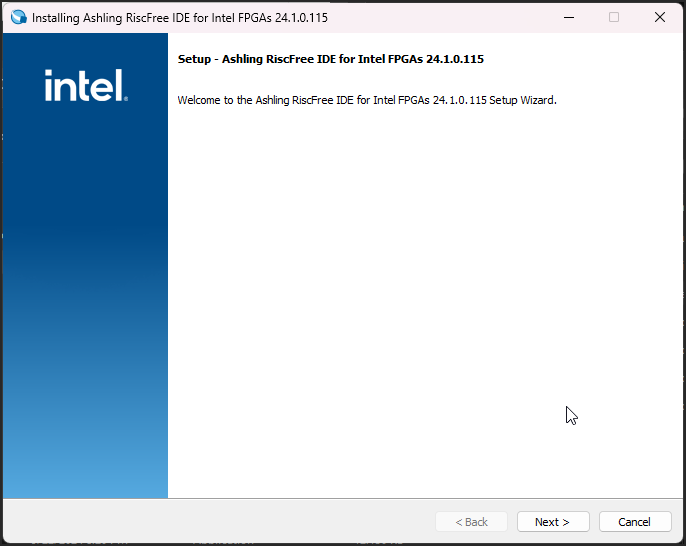
\includegraphics[scale=0.66]{figures/exe3.png}
        \caption{The {\it Ashling RiscFree Software} installation dialogue.}
        \label{fig:exe3}
    \end{center}
\end{figure}

\subsection{Installing the Nios~V Hardware and Software Development Tools}
\label{sec:hw_sw}

This tutorial requires a hardware system containing the Nios~V processor, as well as Nios~V
software development tools for that system. These hardware and software components can be
obtained from {\it GitHub}, at the \texttt{URL} below:

{\href{https://github.com/fpgacademy/Design\_Examples/releases/tag/v1.0} 
{https://github.com/fpgacademy/Design\_Examples/releases/tag/v1.0}.

From the GitHub repository download to your computer the file named {\it fpgacademy.zip}, 
which is listed under \texttt{Assets}. Next, you need to uncompress this {\it ZIP} archive 
file and store its contents into the {\it same} folder where you installed the Quartus 
{\it Programmer Tools} and {\it Ashling RiscFree Software}.

As illustrated in Figure~\ref{fig:goterdone}, your installation folder should now 
contain: the Quartus {\it Programmer Tools} (in the \texttt{qprogrammer} folder), the 
{\it Ashling RiscFree Software} (in the \texttt{riscfree} folder), and the Nios V 
hardware system and software development tools (in the \texttt{fpgacademy} folder).
~\\
\begin{figure}[h]
    \begin{center}
        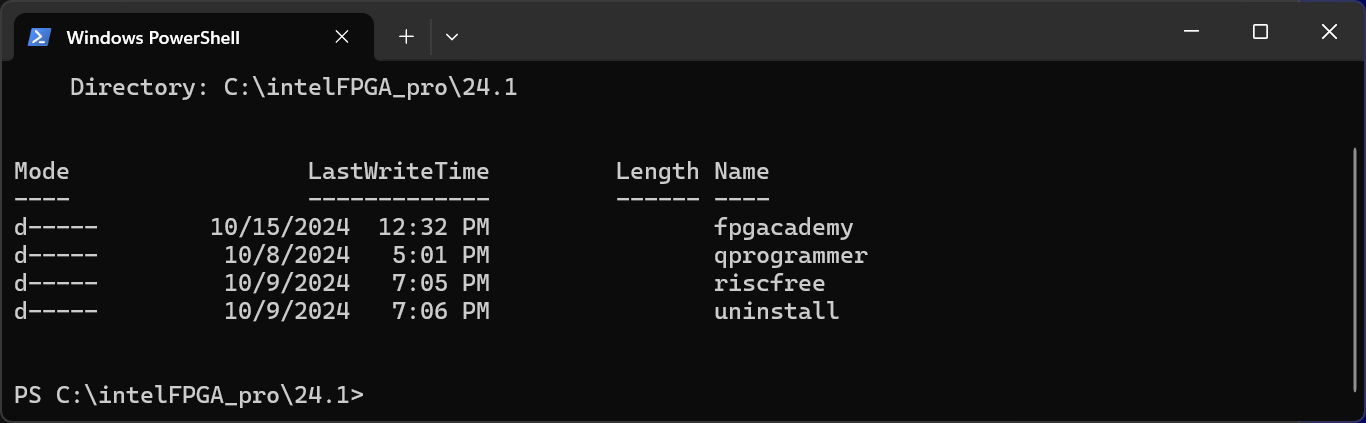
\includegraphics[width=.9\linewidth]{figures/goterdone.png}
        \caption{The final contents of your installation folder.}
        \label{fig:goterdone}
    \end{center}
\end{figure}

\subsection{Installing the Tutorial Design Examples}
\label{sec:egs}

On the {\href{https://www.fpgacademy.org/courses.html} {FPGAcademy.org}} website, this
tutorial is accompanied by {\it Design Files} that are used to illustrate various features
of the {\it GDB} software for developing and debugging Nios~V programs. Download to your 
computer the provided {\it design\_files.zip} file. Then, uncompress this archive into any 
folder of your choice. We will refer to the examples of code and other files in this folder 
throughout the tutorial. Figure~\ref{fig:designfiles} shows the folders included in the
{\it Design Files}, assuming that they have been installed into a folder named
\texttt{GDB\_tutorial}.

\begin{figure}[h]
    \begin{center}
        \includegraphics[width=.9\linewidth]{figures/designfiles.png}
        \caption{The {\it Design Files} folders.}
        \label{fig:designfiles}
    \end{center}
\end{figure}

\section{Setting up the Nios~V Development Environment}
\label{sec:setup}

Once the necessary software and hardware components have been installed onto your computer, 
as discussed in Section~\ref{sec:getthem}, then you can begin working with the {\it GDB}
debugger to develop Nios~V programs. In this tutorial, we use the command-line environment 
provided by the {\it Windows PowerShell}.

\subsection{Using the GNU Make Program}

Open a {\it PowerShell} terminal using a method of your choosing.  Then, navigate to the 
{\it design files} folder called \texttt{C:$\backslash$GDB\_tutorial$\backslash$largest\_s}. 
As illustrated in Figure~\ref{fig:largest1}, this folder contains an example of a 
Nios~V assembly-language program, {\it largest.s}, and a {\it Makefile}. 
~\\
\begin{figure}[h]
    \begin{center}
        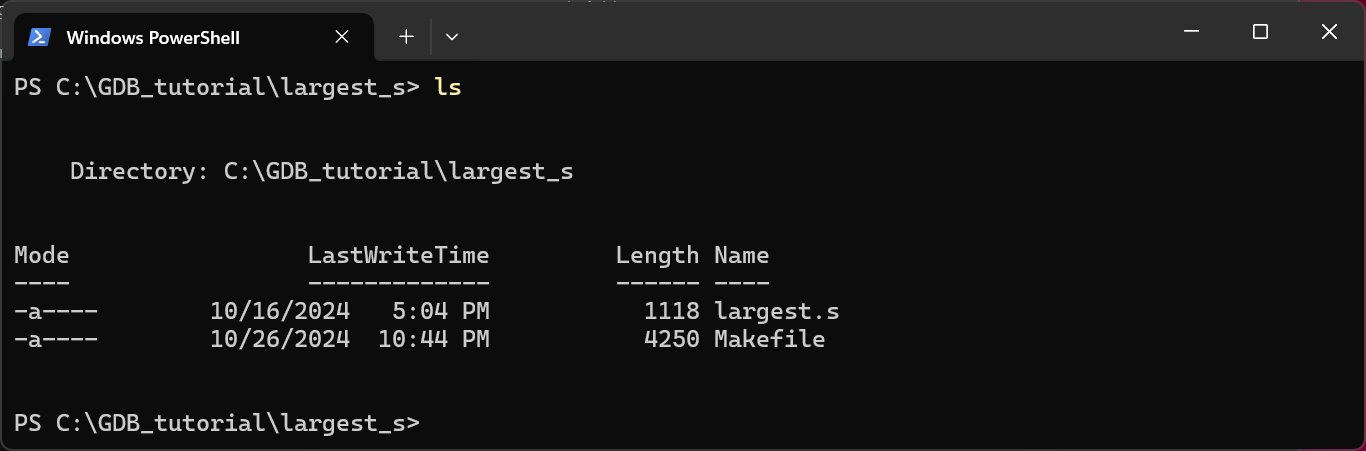
\includegraphics[width=.9\linewidth]{figures/largest1.png}
        \caption{The contents of the largest\_s design files folder.}
        \label{fig:largest1}
    \end{center}
\end{figure}

In this tutorial the tools that we use for developing and debugging Nios~V programs are 
executed via the {\it GNU make} program. A copy of {\it GNU make} is included as part of
the installed software discussed in Section~\ref{sec:getthem}, in the folder:

\texttt{C:$\backslash$intelFPGA\_pro$\backslash$24.1$\backslash$fpgacademy$\backslash$AMP$\backslash$bin}

You should add this folder to your \texttt{Path} {\it Windows Environment Variable}, so
that it is easy to run the {\it make} program.  

\section{Developing and Debugging Nios~V Assembly-Language Programs}
\label{sec:assembly}

In the folder of Figure~\ref{fig:largest1} open the {\it Makefile} in any text editor of your
choice. The first few lines of this file are displayed in Figure~\ref{fig:firstfew}.
Line~1 defines a variable called \texttt{INSTALL} that specifies the folder in which the 
software needed for this tutorial has been installed. The setting given in the figure matches 
the installation folder that we used in Section~\ref{sec:getthem}, as shown in 
Figure~\ref{fig:exe2}. If a different installation folder is used on your computer, then 
change the value of the \texttt{INSTALL} variable accordingly (type forward slashes (/)
as separators to specify the path to your folder, as done in the Figure~\ref{fig:firstfew},
as opposed to backward slashes ($\backslash$)). 

\begin{figure}[h]
    \begin{center}
        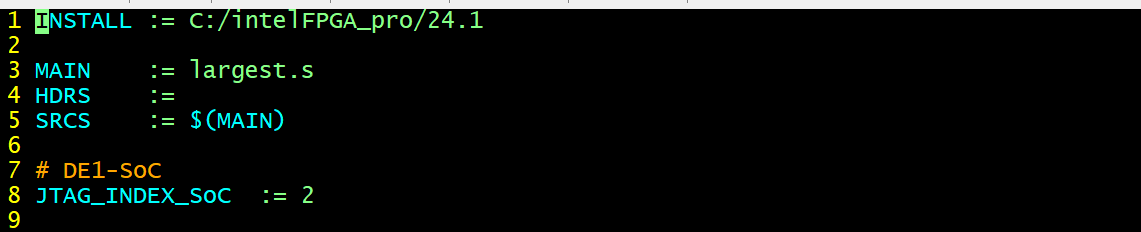
\includegraphics[scale=.5]{figures/firstfew.png}
        \caption{The first few lines of the {\it Makefile}.}
        \label{fig:firstfew}
    \end{center}
\end{figure}

\subsection{Configuring the DE1-SoC Board}

Connect a DE1-SoC board to your computer. The board should be connected by plugging
a cable that has a {\it Type-A USB} connector into the {\it USB Blaster} port on the board 
and connecting the other end of this cable to any {\it USB} port on your computer. Ensure 
that the DE1-SoC board is properly powered on.

To configure your DE1-SoC board with the desired Nios~V computer system, in the terminal
window of Figure~\ref{fig:largest1} execute the command:

\texttt{make DE1-SoC} 

This command runs the Quartus {\it Programmer} and configures the board with the 
{\it DE1-SoC Computer with Nios~V} system. If the command completes without errors, then you 
can skip ahead to Section~\ref{sec:doit} and begin using GDB with Nios~V. 

If the Quartus {\it Programmer} fails to start, then make sure that you have installed the
required software, and that you have properly set up the \texttt{INSTALL} variable shown
in Figure~\ref{fig:firstfew}. If the Quartus {\it Programmer} runs, but fails to configure 
your DE1-SoC board, then try running the command:

\texttt{make DETECT\_DEVICES}

This command checks which devices are visible on the {\it USB Blaster} cable that is connected to
your computer. Part of the expected output from this command is displayed in
Figure~\ref{fig:detect}. It shows 
two devices being detected: first an {\it SOCVHPS} device, followed by a Cyclone V {\it 5CSE} 
{\it FPGA} device.  If the output produced from your board shows these two devices, but in the 
opposite order, then you have to modify your {\it Makefile}.
Change the variable \texttt{JTAG\_INDEX\_SoC} shown in Line~8 of 
Figure~\ref{fig:firstfew} from the value \texttt{2} to the value \texttt{1}. You should now 
be able to successfully configure your DE1-SoC board by executing the \texttt{make DE1-SoC}
command. Another possible scenario is that you are using a board other 
than the DE1-SoC board. If using the DE10-Lite board, then run the 
command \texttt{make DE10-Lite} to configure your board. If you are using some other board, 
then you will need to read carefully through the {\it Makefile} to determine how its
commands have to be modified to suit your board. 

\begin{figure}[h]
    \begin{center}
        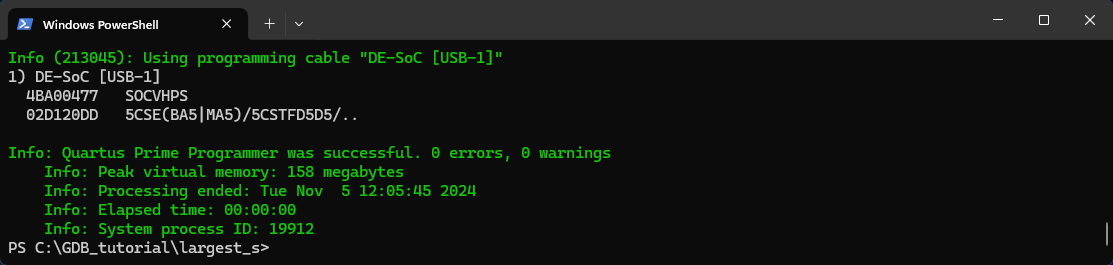
\includegraphics[scale=.55]{figures/detect.png}
        \caption{The output from \texttt{make DETECT\_DEVICES}.}
        \label{fig:detect}
    \end{center}
\end{figure}

\subsection{Using the GDB Server and Client}
\label{sec:doit}

To develop Nios~V programs, you need to use {\bf two} PowerShell terminals: the first one
is used to open the {\it GDB Server}, and the second one is used run the {\it GDB Client}. 
To start the GDB Server, in the terminal window of Figure~\ref{fig:largest1} execute the command:

\texttt{make GDB\_SERVER}

The server will then remain running in this window, as indicated in Figure~\ref{fig:server}. 
Now, open another PowerShell window (you can simply click on the \texttt{+} button near the 
top of Figure~\ref{fig:server} to open a new PowerShell {\it tab}). In this new terminal 
tab navigate again to the same folder as in Figure~\ref{fig:largest1}. 

\begin{figure}[h]
    \begin{center}
        \includegraphics[scale=.55]{figures/server.png}
        \caption{Running the GDB Server.}
        \label{fig:server}
    \end{center}
\end{figure}

This part of the tutorial uses an assembly-language program, {\it largest.s}, which is shown 
in Figure~\ref{fig:largest_code}. This program searches through a list of integers that is 
stored in memory and finds the largest number in the list. Assemble this program by 
executing the command \texttt{make COMPILE}.
You could also just type \texttt{make}, because \texttt{COMPILE} is the first target in the 
{\it Makefile}. As illustrated in Figure~\ref{fig:make_largest}, this command runs the Nios~V
assembler and linker tools to generate the Nios~V executable file {\it largest.elf}.

\begin{figure}[H]
\lstinputlisting[style=defaultNiosVStyle]{Code/largest.s}
	\caption{A program that finds the largest number in a list.}
	\label{fig:largest_code}
\end{figure}

\begin{figure}[h]
    \begin{center}
        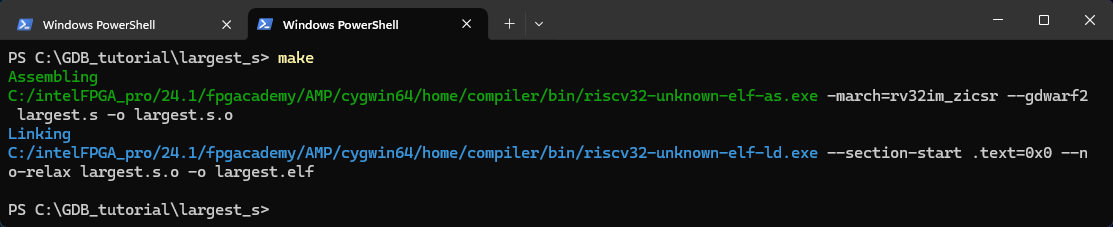
\includegraphics[scale=.55]{figures/make_largest.png}
        \caption{Making the executable file {\it largest.elf}.}
        \label{fig:make_largest}
    \end{center}
\end{figure}

Now you can run the {\it GDB Client} by executing the command:

\texttt{make GDB\_CLIENT}

The GDB Client will connect to your DE1-SoC board, load the executable file {\it largest.elf},
initialize some Nios~V control registers, and set the Nios~V program counter register, {\it pc},
to the start of the program. The output produced by this command is displayed in 
Figure~\ref{fig:gdb_client}.

\begin{figure}[h]
    \begin{center}
        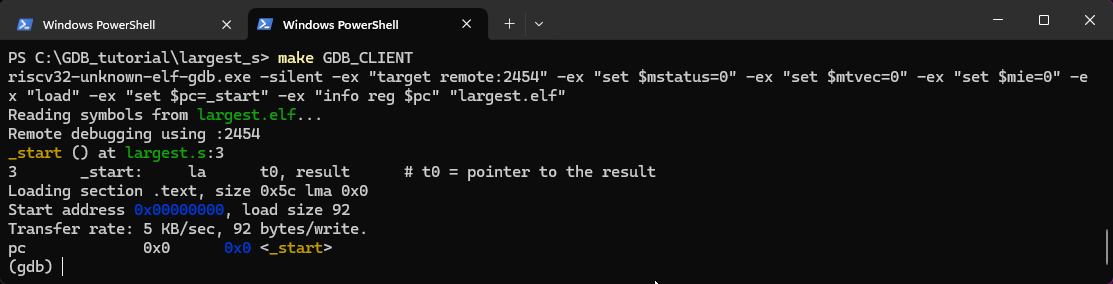
\includegraphics[scale=.6]{figures/gdb_client.png}
        \caption{Starting the GDB Client.}
        \label{fig:gdb_client}
    \end{center}
\end{figure}

We will use the {\it largest.s} program as an example to illustrate some basic GDB commands. 
A summary of the GDB commands used in this tutorial is provided in Appendix A. Of course, a 
lot of documentation about GDB commands can also be found on the Internet. 

In the GDB Client type the \texttt{list} command, as shown in the 
Figure~\ref{fig:gdb1}, to see the loaded program.

\begin{figure}[h]
    \begin{center}
        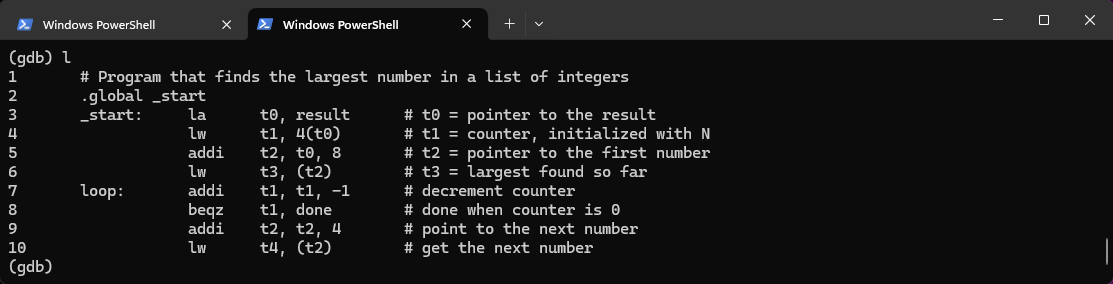
\includegraphics[scale=.6]{figures/gdb1.png}
        \caption{The output of the \texttt{list} command.}
        \label{fig:gdb1}
    \end{center}
\end{figure}

Next, execute the first two instructions in the program by using the 
GDB \texttt{step} command twice. Then, execute the commands 
\texttt{info reg t0} and \texttt{info reg t1} to see that register \texttt{t0} 
holds the address in memory of the \texttt{result} label, which is \texttt{0x38}, and that
register \texttt{t1} has the number of elements in the list, which is \texttt{7} (this value is
specified at the label \texttt{N} in the code in Figure~\ref{fig:largest_code}).
The results of these commands are displayed in Figure~\ref{fig:gdb2}. You can see the
contents of memory by using the \texttt{x} command. Enter \texttt{x/4x result} to see the
four words of memory starting at the address of the \texttt{result} label (\texttt{/4x}
designates four \texttt{words} displayed in \texttt{hexadecimal}).

As illustrated in Figure~\ref{fig:gdb3} set a breakpoint at line 7 in the source code,
which corresponds to the label \texttt{loop}, by using the command \texttt{break 7}.
Then, run to this breakpoint twice by using the \texttt{continue}
command. Check the value of register \texttt{t3} to see that the largest number found in
the list so far is \texttt{5}. 
Now, clear the breakpoint by using the command \texttt{clear 7}. Then, use the
\texttt{continue} command to run to the end of the program, as illustrated in
Figure~\ref{fig:gdb4}.  At this point the program will
be endlessly looping at the label \texttt{stop} in Figure~\ref{fig:largest_code}. To
return control to the GDB Client type $^{\wedge}\texttt{C}$ (hold down the \texttt{CTRL} key 
on your keyboard and press \texttt{c}). 

We are now finished with the {\it largest\_s} example. As demonstrated in Figure~\ref{fig:gdb4},
disconnect from your DE1-SoC board by executing the \texttt{detach} command. Finally, execute
the \texttt{quit} command. If you see the prompt \texttt{Terminate batch job (Y/N)?}
respond with \texttt{n}.

In the GDB Server terminal of Figure~\ref{fig:server}, type \texttt{q} to quit. While
it is not absolutely necessary to exit the server before starting to work on another
Nios~V program, it is a good idea to do so. The server occasionally experiences
communications failures with the DE1-SoC board and then has to be restarted---hence, leaving 
the server running for long periods of time may not be a good approach.
        
~\\
\begin{figure}[h]
    \begin{center}
        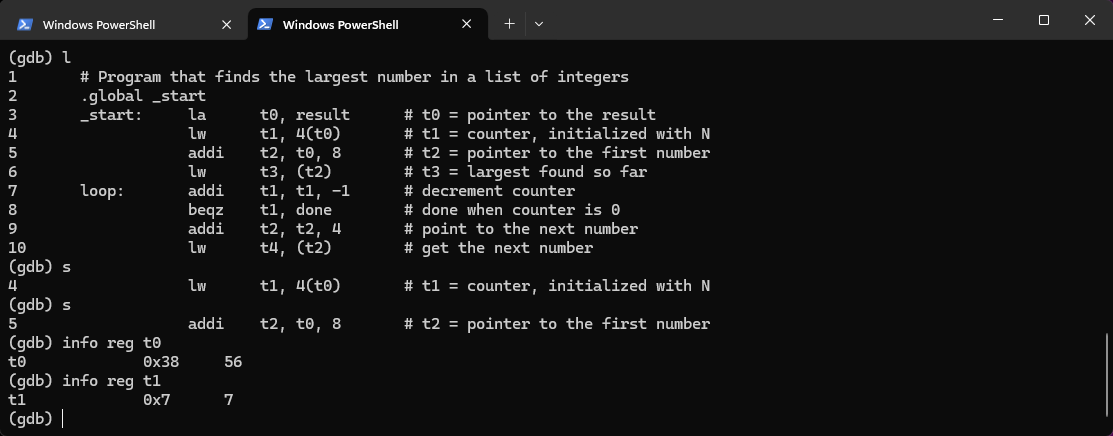
\includegraphics[scale=.6]{figures/gdb2.png}
        \caption{Executing a few GDB commands.}
        \label{fig:gdb2}
    \end{center}
\end{figure}


\begin{figure}[h]
    \begin{center}
        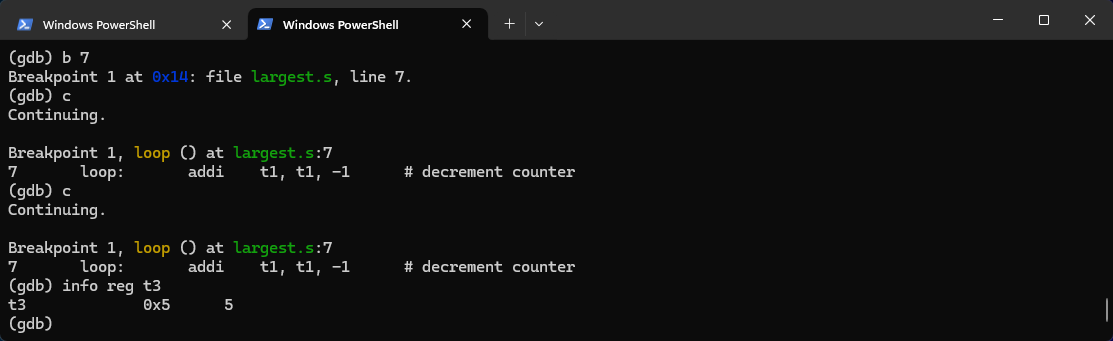
\includegraphics[scale=.6]{figures/gdb3.png}
        \caption{Using a breakpoint.}
        \label{fig:gdb3}
    \end{center}
\end{figure}

\begin{figure}[h]
    \begin{center}
        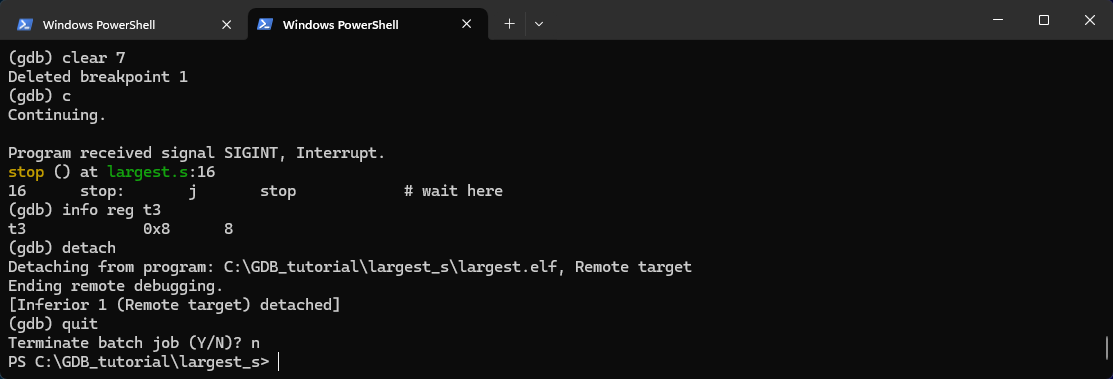
\includegraphics[scale=.6]{figures/gdb4.png}
        \caption{Completing the program and quitting from GDB.}
        \label{fig:gdb4}
    \end{center}
\end{figure}

\section{Design Files Examples}

Having learned the basics about using GDB with Nios~V in Section~\ref{sec:doit}, we will 
now utilize the various design files examples provided with this tutorial to illustrate
additional GDB capabilities. 

\subsection{Using Simple I/O Devices with Assembly Code}
\label{sec:simpleIO}

When starting to work on a new design example it is a good approach to power your DE1-SoC
board \texttt{off}, and then \texttt{on} again, so that the system is reset.   
Open a PowerShell terminal and navigate to the folder for the \texttt{display\_s} design
example. In this folder, execute the command \texttt{make DE1-SoC} to configure your board. 
If this programming step fails, refer to the discussion in Section~\ref{sec:doit} for
suggestions as to how to fix any issues. Once your board is successfully configured,
execute the command \texttt{make GDB\_SERVER}. Now, open a second
PowerShell tab (as described in Section~\ref{sec:doit}) and, as illustrated in 
Figure~\ref{fig:display_s1}, navigate again to the \texttt{display\_s} folder and 
execute the command \texttt{make COMPILE}, followed by \texttt{make GDB\_CLIENT}.

\begin{figure}[h]
    \begin{center}
        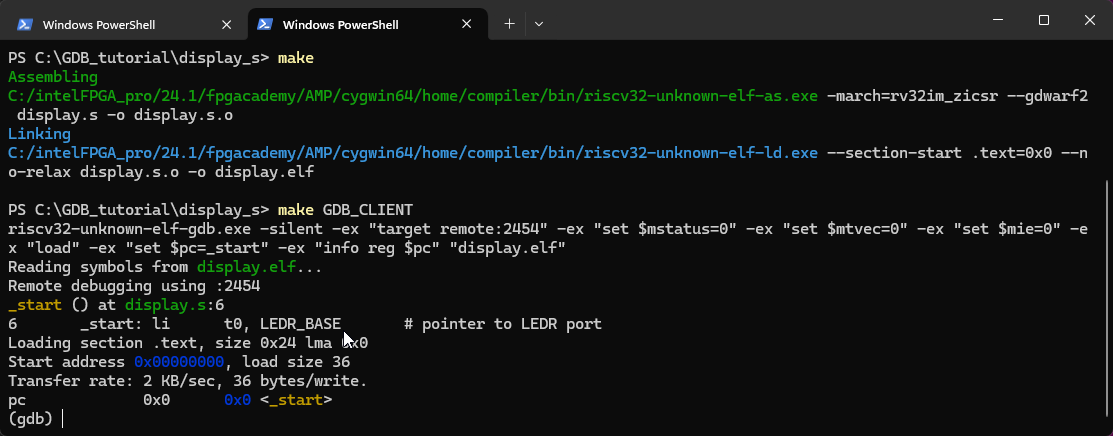
\includegraphics[scale=.6]{figures/display_s1.png}
        \caption{Starting GDB for the \texttt{display\_s} example.}
        \label{fig:display_s1}
    \end{center}
\end{figure}

Within the GDB Client, use \texttt{list 1,14} to see the source-code of the program. As
shown in  Figure~\ref{fig:display_s2}, the program first sets up three pointers to I/O
devices in the {\it DE1-SoC Computer}: register {\it t0} is initialized to the address of 
the \red{{\it LEDR}} red light port, register {\it t1} to the address of the {\it SW} slide-switch
port, and register {\it t2} to the address of the port connected to 7-segment display 
\red{{\it HEX3}} to \red{{\it HEX0}}. The program then executes an endless loop in 
which it loads the current value of the {\it SW} switch port and stores this value to 
both the \red{{\it LEDR}} and \red{\it HEX0}} display ports. 

Run the program by executing the \texttt{continue} command. While the program is running,
experiment with different settings on the {\it SW}$_{6-0}$ switches on the DE1-SoC board and observe 
the \red{{\it LEDR}} lights and \red{{\it HEX0}} display. 

Type $^{\wedge}\texttt{C}$ to stop the running program and return control to the GDB
Client. Now, set a breakpoint at the top of the \texttt{loop} in the program with the
command \texttt{break 10}. Use the \texttt{continue} command to run the program to the
breakpoint at \texttt{Line 10} (at the label \texttt{loop}). Set a desired pattern on 
the {\it SW} switches and then execute the \texttt{step} command,
followed by \texttt{info reg t3} to see the value loaded from the {\it SW} port. Execute 
\texttt{step} again and observe the \red{{\it LEDR}} lights, then use \texttt{step} again and 
observe the \red{{\it HEX0}} display. 

\begin{figure}[h]
    \begin{center}
        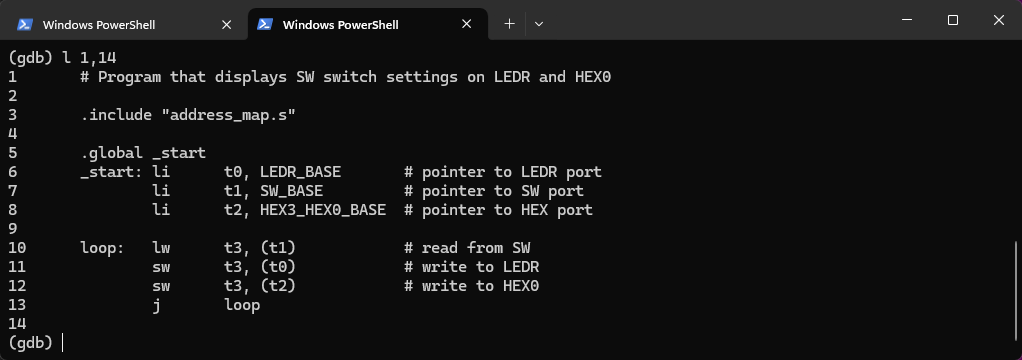
\includegraphics[scale=.6]{figures/display_s2.png}
        \caption{The \texttt{list} command.}
        \label{fig:display_s2}
    \end{center}
\end{figure}

Use \texttt{continue} again to get to the top of the loop, and then \texttt{step} to
execute the {\it load} instruction at \texttt{Line 10}. Now, use the GDB command 
\texttt{set \$t3 = 0x3ff} to overwrite the value loaded into register {\it t3}. Use
\texttt{step} again and then observe on the DE1-SoC board that the value you placed 
into register {\it t3} turns on all ten \red{{\it LEDR}} lights. 

We are now done with this design example, so use the \texttt{detach} command to disconnect
from the DE1-SoC board. Finally, \texttt{quit} from the GDB Client, and then go to the
GDB Server PowerShell tab and type \texttt{q} to close the server.

\subsection{Using Interrupts with Assembly Code}

The assembly code example for this part of the tutorial displays a one-second binary counter on 
the red lights \red{{\it LEDR}}. The speed of the counter is controlled by using interrupts from 
the Nios~V Machine Timer.  

Open a PowerShell terminal and navigate to the \texttt{interrupt\_s} folder.
If not already done, configure your DE1-SoC board by running \texttt{make DE1-SoC}. Execute 
\texttt{make GDB\_SERVER}. In a second PowerShell tab navigate again to the 
\texttt{interrupt\_s} folder and run \texttt{make COMPILE} and \texttt{make GDB\_CLIENT}.

In the GDB Client, as illustrated in Figure~\ref{fig:interrupt_s1}, run \texttt{list 1,15}. 
Use \texttt{step} to execute the instruction on \texttt{Line 5} that initializes the stack pointer
register. Next, enter \texttt{x/4x 0xff202100}. This command displays the contents 
of the memory-mapped 64-bit Nios~V \texttt{Machine Timer} registers, which are referred to as 
{\it mtime}, which has the address \texttt{0xff202100}, and {\it mtimecmp}, which has the
address \texttt{0xff202108}.

Next, set a breakpoint using \texttt{break 9}. Then, execute \texttt{continue}, which runs the
Nios~V program to call the subroutine {\it set\_timer} and then stops, after returning, at 
the breakpoint on \texttt{Line 9}. Again, as illustrated in Figure~\ref{fig:interrupt_s2}, use 
\texttt{x/4x~0xff202100} to display the Machine Timer registers. As indicated in the figure, 
the {\it mtime} register was cleared to 0 (and then continued counting up at its 100 MHz clock 
rate), and the {\it mtimecmp} register was set to 100,000,000 (\texttt{0x5f5e100}) to
provide machine timer timeouts for every one second.  

\begin{figure}[h]
    \begin{center}
        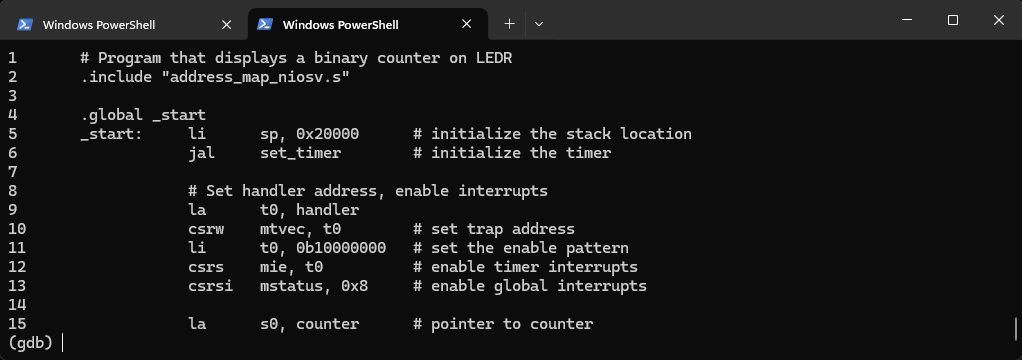
\includegraphics[scale=.6]{figures/interrupt_s1.png}
        \caption{The \texttt{interrupt\_s} example.}
        \label{fig:interrupt_s1}
    \end{center}
\end{figure}

\begin{figure}[h]
    \begin{center}
        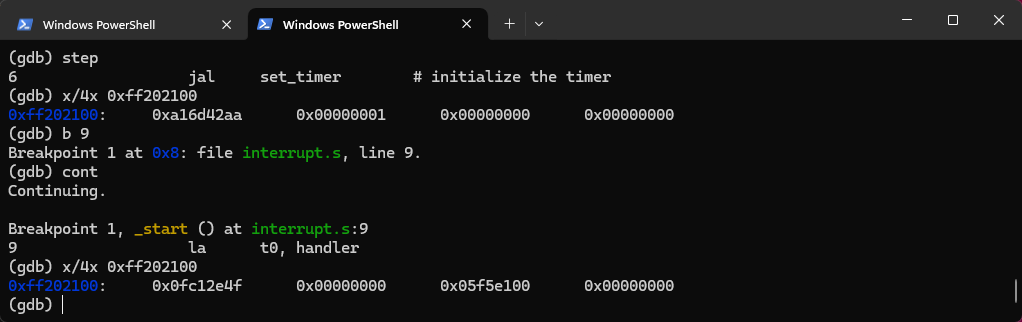
\includegraphics[scale=.6]{figures/interrupt_s2.png}
        \caption{Examining the Nios~V Machine Timer registers.}
        \label{fig:interrupt_s2}
    \end{center}
\end{figure}

The next five instructions in the program set up Nios~V interrupts as needed for this
example. As shown in Figure~\ref{fig:interrupt_s3}, display
the contents of the (uninitialized) {\it mtvec} control register by using
\texttt{info reg mtvec}. Enter \texttt{step 2} to execute two instructions, and
then use \texttt{info reg mtvec} to see that this register has been initialized to
\texttt{0x68}. Enter \texttt{info symbol 0x68} to see that this is the address in memory of the 
interrupt {\it handler} routine. 
Display the current contents of the {\it mie} and {\it mstatus} control registers
with \texttt{info reg mie status}. Execute three more instructions (\texttt{step 3}) and
then enter \texttt{info reg mie mstatus} again to see that the {\it mie} register now
contains the value \texttt{0x80}, which has the interrupt-enable bit corresponding to the
Machine Timer set to 1, and {\it mstatus} shows that the {\it Machine-mode Interrupt Enable} bit
({\it MIE}) in this register is now set to 1, meaning that Nios~V interrupts are now
enabled ({\it Machine} mode is the only processor mode supported in Nios~V).

\begin{figure}[h]
    \begin{center}
        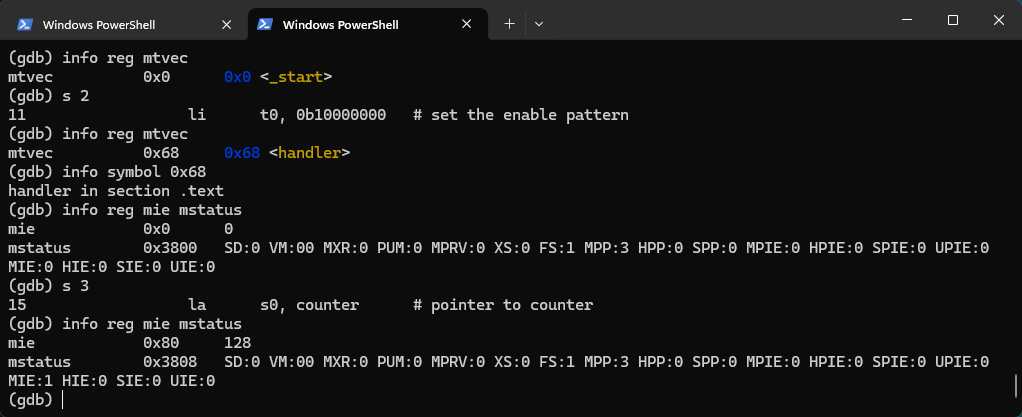
\includegraphics[scale=.6]{figures/interrupt_s3.png}
        \caption{Examining Nios~V control registers.}
        \label{fig:interrupt_s3}
    \end{center}
\end{figure}

Clear the breakpoint that was previously set by entering \texttt{clear 9}. 
Enter \texttt{continue} to run the program and observe that the \red{{\it LEDR}} lights
show a binary counter incrementing once per second. Type $^{\wedge}\texttt{C}$ to
interrupt the program and return control to the GDB Client.

Next, enter \texttt{break handler} to set a breakpoint at the interrupt handler routine.
Note that this code is in a different source-code file, {\it handler.s}, from the main program.
Enter \texttt{continue} to run the program until it reaches the breakpoint. Enter
\texttt{list} to see the first few lines of code in the {\it handler} routine, as displayed in
Figure~\ref{fig:interrupt_s4}. Execute the five instructions displayed in the figure, using
\texttt{step 5}. Then, enter \texttt{info reg t0} to see the cause of the interrupt
(contents of the {\it mcause} control register). The displayed value \texttt{0x80000007}, as 
seen in Figure~\ref{fig:interrupt_s5}, shows that a hardware interrupt has occurred (\texttt{0x8})
from the device with interrupt number \texttt{7}. This is the expected result, as
interrupt 7 corresponds to the Machine Timer. 

Clear the handler interrupt by entering \texttt{clear handler}, and then \texttt{continue}
execution of the program. Observe the \red{{\it LEDR}} lights to get an indication of the
value of the binary {\it counter} being displayed. Type $^{\wedge}\texttt{C}$ to stop the
program and return control to the GDB Client. To see the current value of the {\it counter}
use the command \texttt{x counter}. It is possible to change the value of this ``variable'' 
by using the \texttt{set} command. For example, set the counter to the value \texttt{0x3f0} by
using \texttt{set \{int\} counter = 0x3f0}. The cast to type \texttt{\{int\}} is required so that 
GDB knows the {\it type} of the variable. Enter continue and observe the new value of
the counter displayed on the \red{{\it LEDR}} lights. Another way to modify the value of
the counter is to first find its address with the command \texttt{info address counter}.
This command returns the address value \texttt{0x64}. Thus, an alternative way to set the 
counter to the value \texttt{0x3f0} is to used the command
\texttt{set *0x64 = 0x3f0}. Here \texttt{*0x64}
uses the syntax of the C language to set the {\it contents} of an address ({\it pointer}). 

\begin{figure}[h]
    \begin{center}
        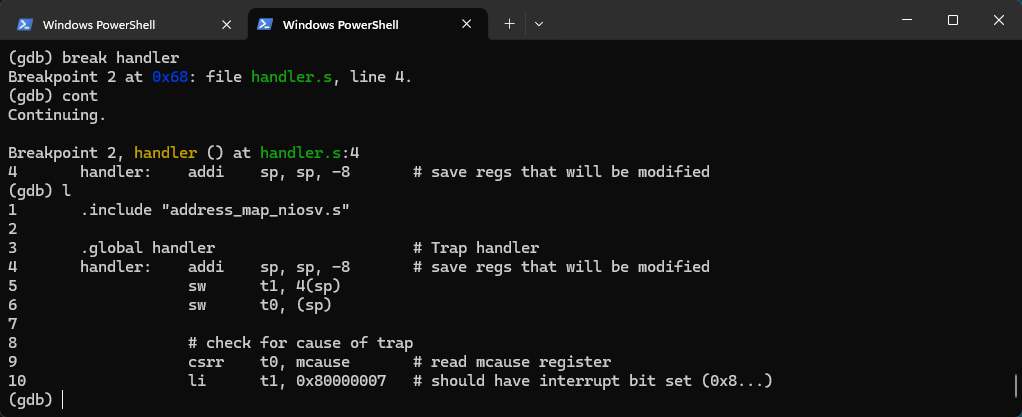
\includegraphics[scale=.6]{figures/interrupt_s4.png}
        \caption{The interrupt {\it handler} routine.}
        \label{fig:interrupt_s4}
    \end{center}
\end{figure}

\begin{figure}[h]
    \begin{center}
        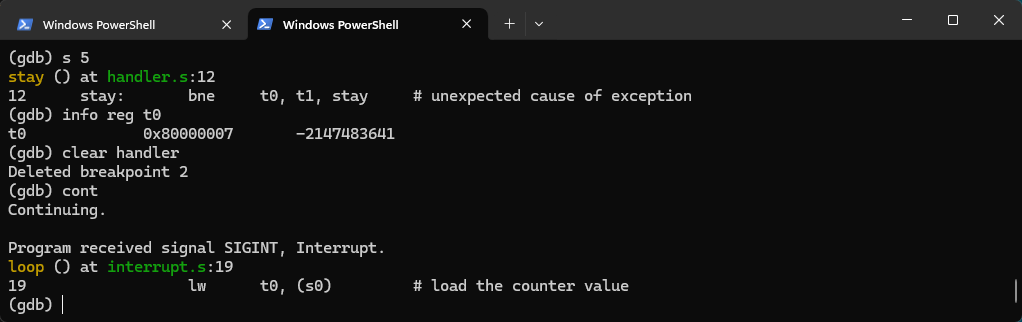
\includegraphics[scale=.6]{figures/interrupt_s5.png}
        \caption{Checking the cause of the interrupt.}
        \label{fig:interrupt_s5}
    \end{center}
\end{figure}

We are now finished with this example, so enter \texttt{detach} to close the connection between 
the GDB Client and the DE1-SoC board, and then enter \texttt{quit}.

\subsection{Using a Terminal to Print Text Messages from Assembly Code}

As a final example using assembly language, we will show how you can ``print'' text messages 
to a terminal window.  This example can be found in the design files folder 
\texttt{JTAG\_UART\_s}. As done previously, open two PowerShell terminals and navigate to
the proper folder. In one terminal
start the GDB Server. In the other terminal, execute \texttt{make} to build the program's
executable file, and then start the GDB Client. Now, open a {\it third} PowerShell
terminal and navigate again to the \texttt{JTAG\_UART\_s} folder. Execute the command 
\texttt{make TERMINAL}. This command creates a communications link between the PowerShell
terminal and the JTAG UART on the DE1-SoC board, which can be used to display text
messages. 

In the GDB Client run the assembly program by entering \texttt{continue}. Observe that the
message 

\texttt{JTAG UART example code}

appears in the terminal that is connected to the
JTAG UART. Also, on a separate line the \texttt{>} prompt is shown. Click on this line,
and then type some text with your keyboard. The text is simply echoed back to the terminal
window by the assembly program that is running. 

In the GDB Client type $^{\wedge}\texttt{C}$ to stop the program. Then, to see how GDB can
be used to restart a program enter the command \texttt{set \$pc = \_start}, or
(equivalently) \texttt{set \$pc = 0}. Use \texttt{continue} to restart the program and 
observe the JTAG terminal window. 

Finally, \texttt{detach} from the GDB Client and \texttt{quit}. Then, close the PowerShell
terminal connected to the JTAG UART, and also stop the GDB Server.
Close the connection to the JTAG terminal by typing $^{\wedge}\texttt{C}$ in its window.

\subsection{Using I/O Devices with C Code}

In this part of the tutorial we will use GDB to run a C program that accesses some simple 
I/O devices. As in previous examples, open two PowerShell terminals. In each terminal 
navigate to the folder for this design example, which is \texttt{display\_C}. Use one 
terminal to start the GDB server. In the other terminal first execute \texttt{make}, which 
builds the executable program by running the C compiler and linker, and then start the GDB 
Client, as shown in Figure~\ref{fig:display_C0}.

Within the GDB Client enter \texttt{break main}, and then run the program using \texttt{continue}.
Type \texttt{list} to see the beginning part of the main program for this example, as displayed in 
Figure~\ref{fig:display_C1}.

Enter \texttt{break 15} to set a breakpoint, and then use \texttt{continue} to run to 
Line 15 in the source code. On the DE1-SoC board, set the {\it SW} switches to any value of
your choosing, for example \texttt{0x7f}. Use \texttt{step} to execute the C statement on
Line 15, and then execute \texttt{print /x value} to examine the data that was loaded, as 
depicted in Figure~\ref{fig:display_C2}. To see which Nios~V register is used to hold
this data, execute the \texttt{disassemble} command. As illustrated in 
Figure~\ref{fig:display_C3}, register {\it a5} is used to hold this {\it value}. Display
the contents of this register by entering \texttt{info reg a5}, as seen in 
Figure~\ref{fig:display_C4}. Use \texttt{step} to execute the next instruction, and
observe that the \red{{\it LEDR}} lights are updated. Then, enter \texttt{continue} to run
the program until it reaches the breakpoint again at Line 15. Observe that the 
\red{{\it HEX0}} display is now updated.

Enter the command \texttt{info break} to see the two breakpoints that are currently set,
at Line 12 ({\it main}) and Line 15. Use the \texttt{delete} command to clear these
breakpoints. 

As we are finished with this example, use \texttt{detach} to disconnect from the DE1-SoC 
board and then \texttt{quit} from the GDB client. In the GDB Server terminal type 
\texttt{q} to quit.

\begin{figure}[h]
    \begin{center}
        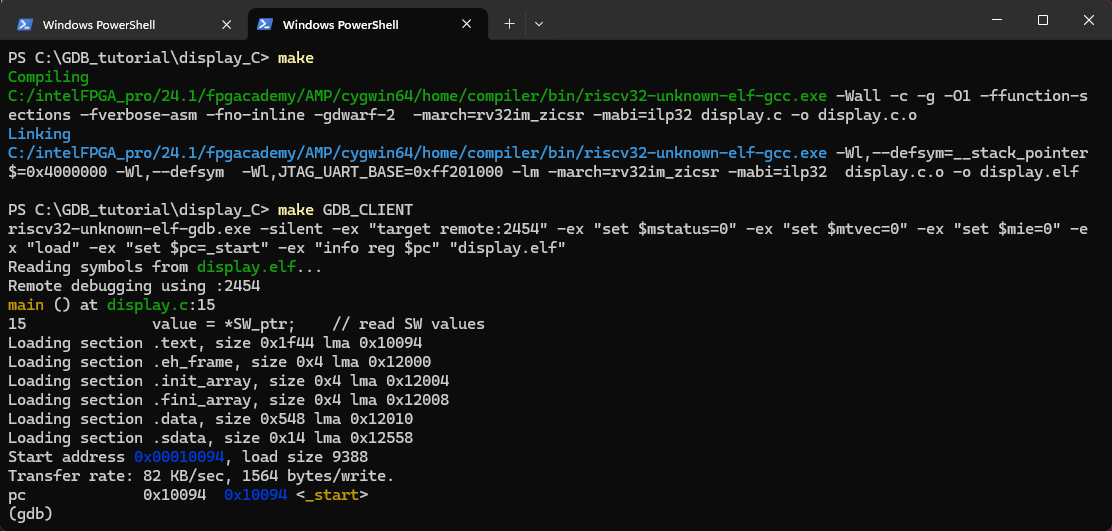
\includegraphics[scale=.6]{figures/display_C0.png}
        \caption{Starting GDB for the \texttt{display\_C} example.}
        \label{fig:display_C0}
    \end{center}
\end{figure}

\begin{figure}[h]
    \begin{center}
        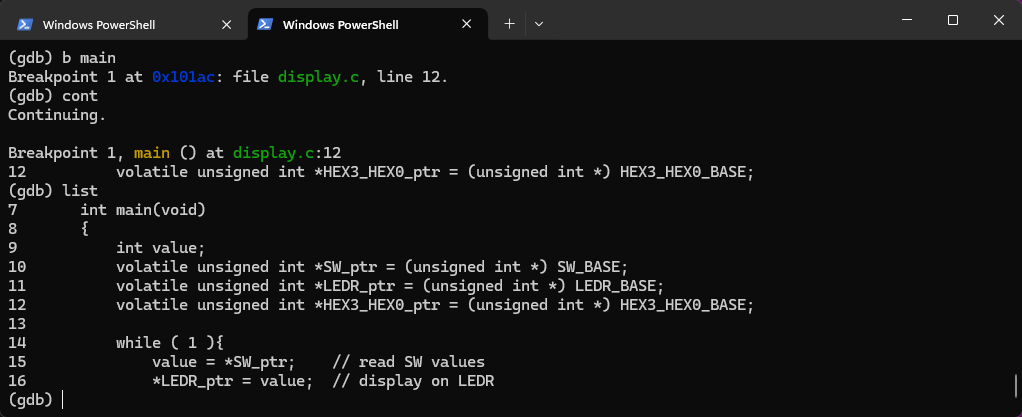
\includegraphics[scale=.6]{figures/display_C1.png}
        \caption{Listing the {\it main} function.}
        \label{fig:display_C1}
    \end{center}
\end{figure}

\begin{figure}[H]
    \begin{center}
        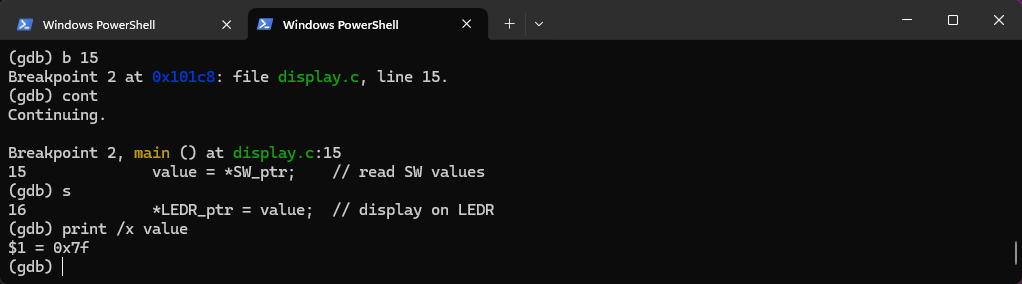
\includegraphics[scale=.6]{figures/display_C2.png}
        \caption{Loading a variable from an I/O device.}
        \label{fig:display_C2}
    \end{center}
\end{figure}

\begin{figure}[H]
    \begin{center}
        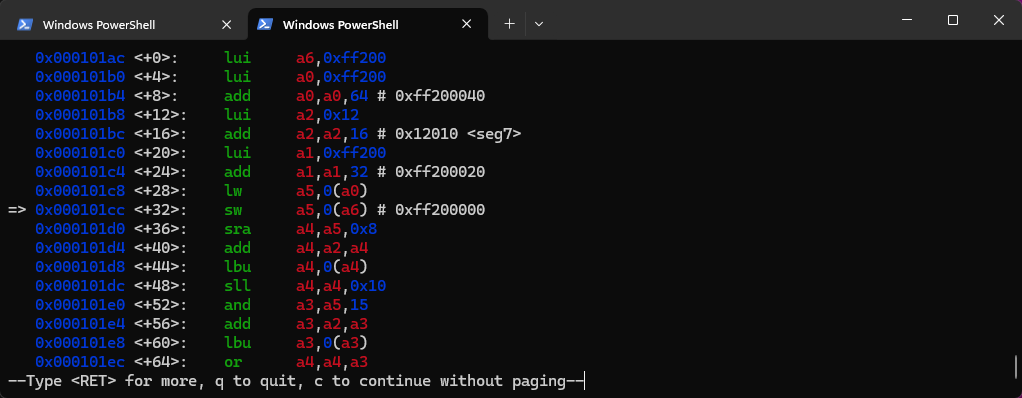
\includegraphics[scale=.6]{figures/display_C3.png}
        \caption{Disassembling C code into assembly code.}
        \label{fig:display_C3}
    \end{center}
\end{figure}

\begin{figure}[H]
    \begin{center}
        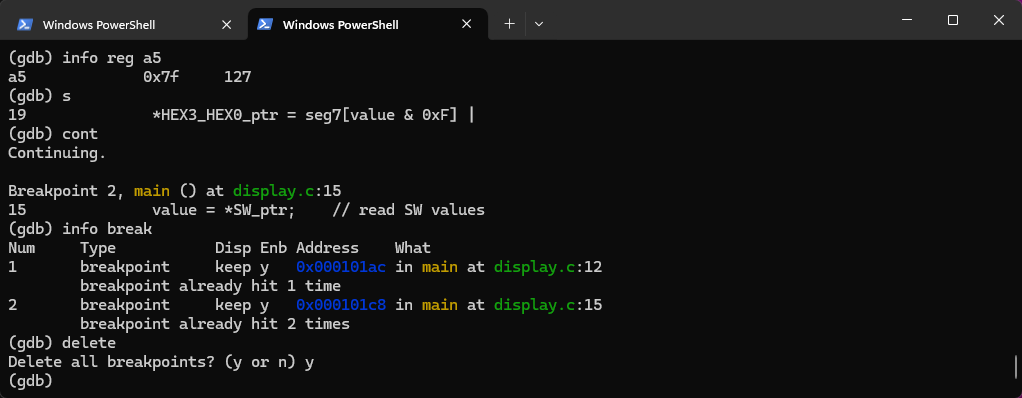
\includegraphics[scale=.6]{figures/display_C4.png}
        \caption{Stepping through C code.}
        \label{fig:display_C4}
    \end{center}
\end{figure}

\subsection{Using Interrupts with C Code}

This part of the tutorial uses Nios~V interrupts with C code. 
As in previous examples, open two PowerShell terminals. In each terminal 
navigate to the folder for this design example, which is \texttt{interrupt\_C}. Use one 
terminal to start the GDB server. In the other terminal first execute \texttt{make}, which 
builds the executable program by running the C compiler and linker, and then start the GDB 
Client.

Within the GDB Client enter \texttt{break main}, and then run the program using \texttt{continue}.
Enter \texttt{list 37,46} to see the beginning part of the main program for this example, as 
displayed in Figure~\ref{fig:interrupt_C1}.

\begin{figure}[h]
    \begin{center}
        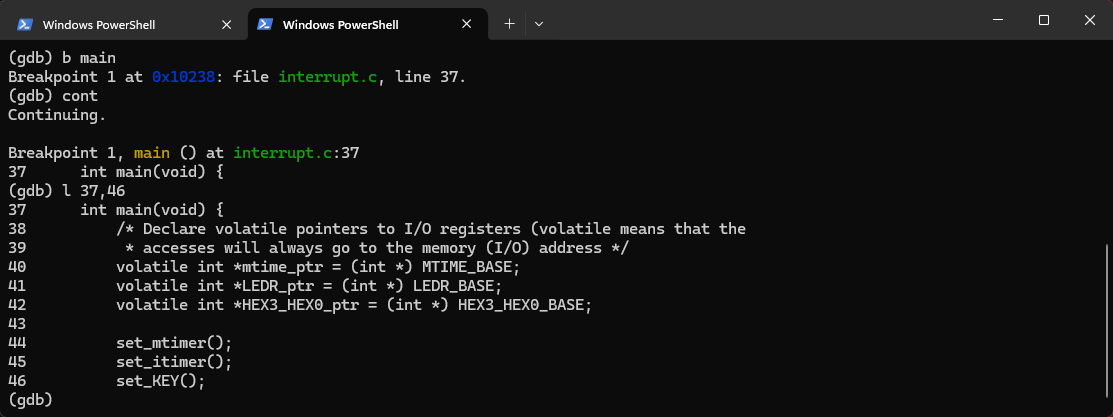
\includegraphics[scale=.6]{figures/interrupt_C1.png}
        \caption{The {\it main} function.}
        \label{fig:interrupt_C1}
    \end{center}
\end{figure}

Execute the \texttt{break 44} command and then use \texttt{continue} to run to Line 44 of the 
source code. Before executing the subroutine \texttt{set\_mtimer()} in the program, use the
command \texttt{x/4x mtime\_ptr}, as depicted in Figure~\ref{fig:interrupt_C2}, to observe the
current contents of the Nios~V Machine Timer registers. These registers are referred to as
{\it mtime} and {\it mtimecmp}, as described in Section~\ref{sec:simpleIO}. Now, execute the
GDB command \texttt{next}, which causes Nios~V to execute the \texttt{set\_mtimer()} subroutine
in the C program and then return. The \texttt{set\_mtimer()} subroutine sets up the
Machine Timer for one-second timeouts by reading the value of the {\it mtime} register, 
adding 100,000,000 to it, and then storing this result into {\it mtimecmp}. The
{\it mtime} register then continues to increment at its 100 MHz clock rate. Rerun the 
command \texttt{x/4x mtime\_ptr} to see the updated values of the Machine Timer registers. 

\begin{figure}[h]
    \begin{center}
        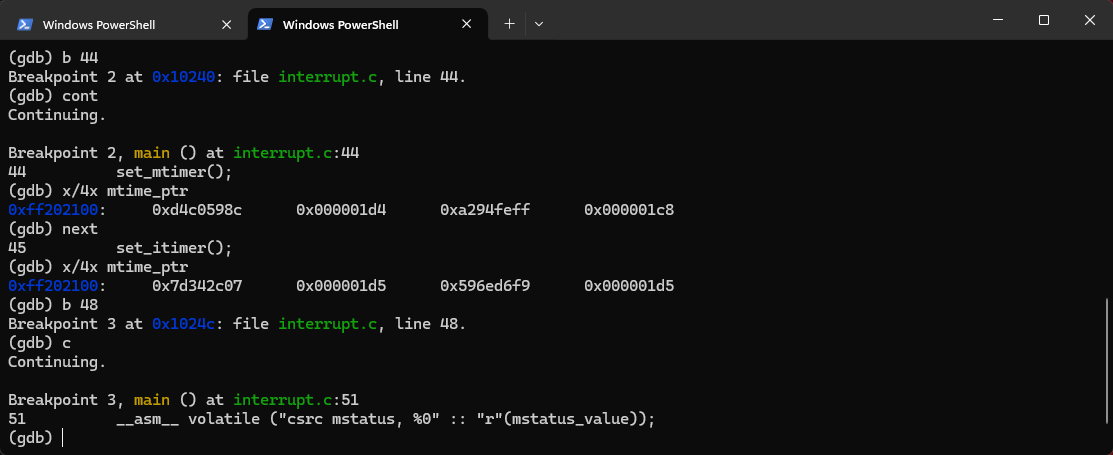
\includegraphics[scale=.6]{figures/interrupt_C2.png}
        \caption{Setting the Machine Timer registers.}
        \label{fig:interrupt_C2}
    \end{center}
\end{figure}

\begin{figure}[h]
    \begin{center}
        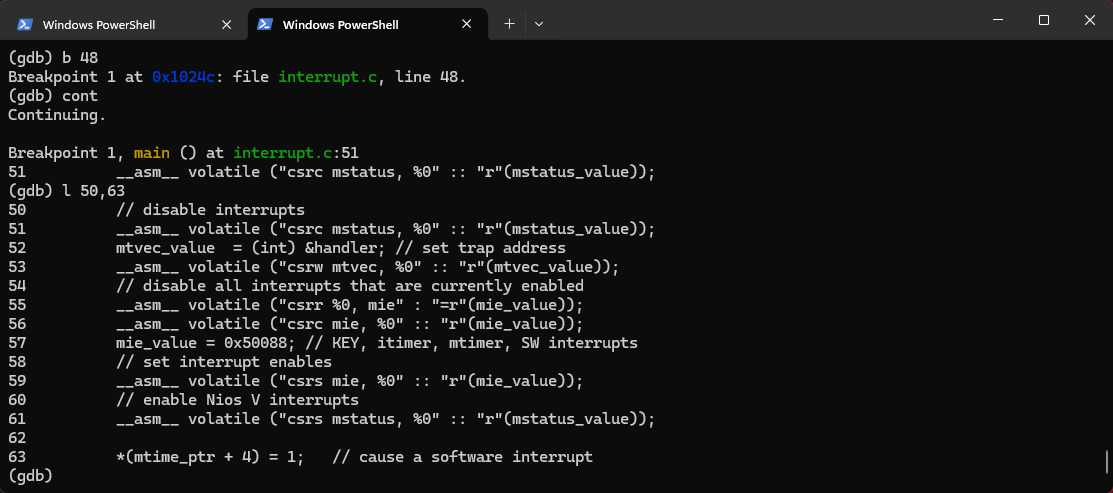
\includegraphics[scale=.6]{figures/interrupt_C3.png}
        \caption{Setting up interrupts.}
        \label{fig:interrupt_C3}
    \end{center}
\end{figure}

Enter \texttt{break 48} and then \texttt{continue} to Line 48. Then, use \texttt{list 50,63}
to show the lines of code displayed in Figure~\ref{fig:interrupt_C3}. The {\it inline
assembly} code shown in the figure sets up Nios~V interrupts as needed for the program.
Use the command \texttt{info reg mstatus mtvec mie} to display the current values of the
pertinent registers. Run the program up to Line 63 and then rerun the command
\texttt{info reg mstatus mtvec mie} to see the updated register values. The {\it mstatus}
register shows that Nios~V interrupts are now enabled for machine mode, and the {\it mtvec}
register contains the address of the interrupt \texttt{handler} routine. The {\it mie}
register has bits set that enable several sources of interrupts: Nios~V software interrupts, 
machine timer, FPGA interval timer, and {\it KEY} push-buttons.

\begin{figure}[h]
    \begin{center}
        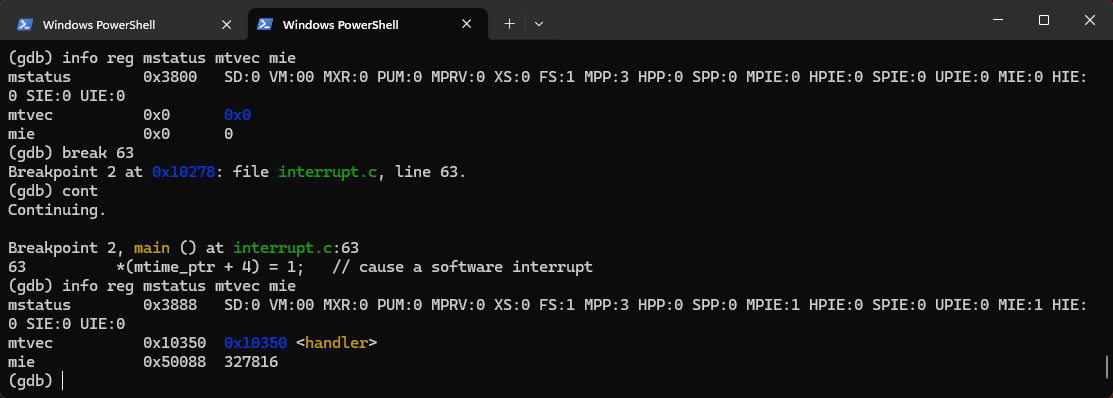
\includegraphics[scale=.6]{figures/interrupt_C4.png}
        \caption{Nios~V control registers.}
        \label{fig:interrupt_C4}
    \end{center}
\end{figure}

\begin{figure}[h]
    \begin{center}
        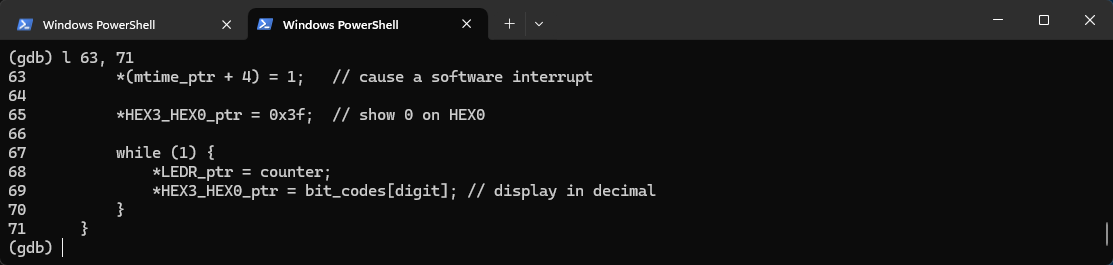
\includegraphics[scale=.6]{figures/interrupt_C5.png}
        \caption{The main program loop.}
        \label{fig:interrupt_C5}
    \end{center}
\end{figure}

Use the command \texttt{list 63, 71} to see the remainder of the {\it main} program. As shown in
Figure~\ref{fig:interrupt_C5}, it contains a 
loop that reads two variables from memory, called {\it counter} and {\it digit}.  The
{\it counter} variable is displayed in binary on the \red{{\it LEDR}} lights, and a decimal 
number is displayed on \red{{\it HEX0}} based on the value of the {\it digit} variable.
Both of these variables are updated by interrupt service routines that respond to hardware 
timers.

The interrupt {\it handler} for this program is given in Figure~\ref{fig:interrupt_code}.
It uses assembly code to read the contents of the Nios~V {\it mcause} control register, and then
uses this value to call the appropriate interrupt service routine. Assume that we wish to
trace the execution of the program when an {\it interval timer} interrupt occurs. In the
GDB Client enter the command \texttt{break itimer\_ISR}. Type \texttt{continue}. When the
breakpoint has been reached, enter \texttt{list}, as displayed in
Figure~\ref{fig:interrupt_C6}. Type {\it step} to execute the next line of code, as
depicted in Figure~\ref{fig:interrupt_C7}. To see the value of the {\it KEY\_dir} variable
loaded by the program enter \texttt{print KEY\_dir}. Type \texttt{step} to update the
\texttt{digit} variable. Typing \texttt{step} again returns from this interrupt service
routine to the interrupted program.

\begin{figure}[H]
\lstinputlisting[language=C, firstline=14, lastline=30]{Code/handlers.c}
	\caption{The interrupt handler.}
	\label{fig:interrupt_code}
\end{figure}

\begin{figure}[h]
    \begin{center}
        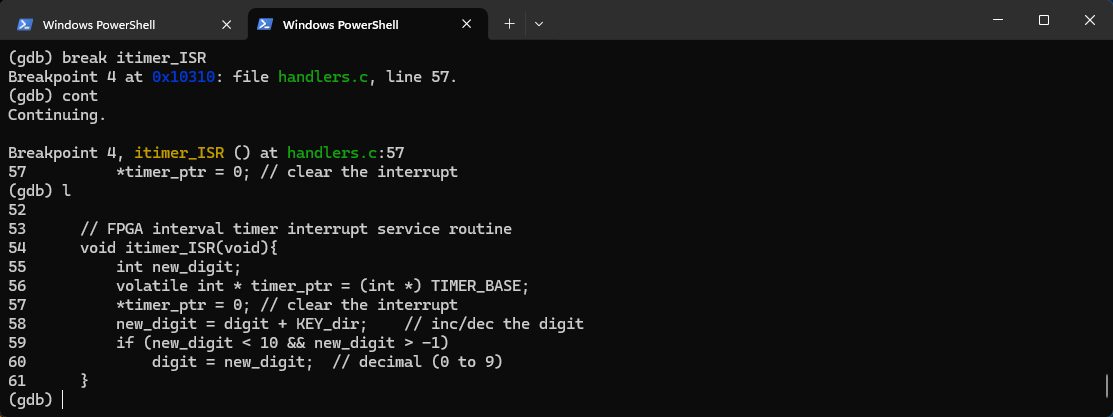
\includegraphics[scale=.6]{figures/interrupt_C6.png}
        \caption{A breakpoint at an interrupt service routine.}
        \label{fig:interrupt_C6}
    \end{center}
\end{figure}

\begin{figure}[h]
    \begin{center}
        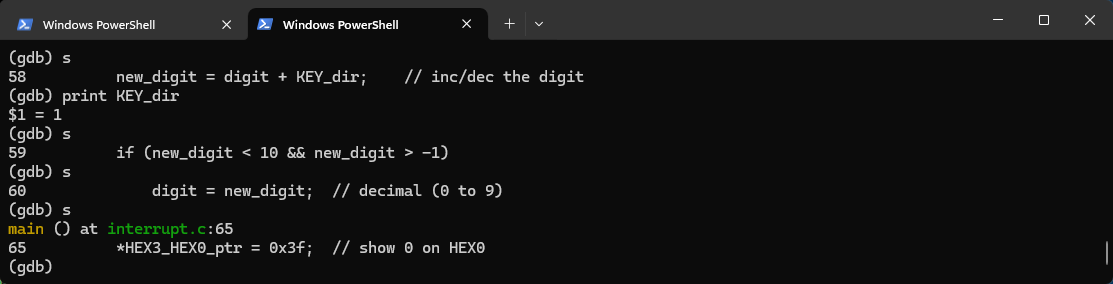
\includegraphics[scale=.6]{figures/interrupt_C7.png}
        \caption{Servicing an interval timer interrupt.}
        \label{fig:interrupt_C7}
    \end{center}
\end{figure}

We are now finished with this example, so use \texttt{detach} to disconnect from the DE1-SoC 
board and then \texttt{quit} from the GDB client. Also, quit from the GDB Server in its 
terminal window. 

\subsection{Using a Terminal to Print from C Code}

As a final example we will show how you can use {\it printf} in C code from within the GDB 
Client.  This example can be found in the \texttt{print\_C} design files folder.
As in previous examples, open two PowerShell terminals. In each terminal 
navigate to the folder for this design example. Use one 
terminal to start the GDB server. In the other terminal first execute \texttt{make} to
build the executable program, and then start the GDB Client.
Now, open a {\it third} PowerShell terminal and navigate again to the \texttt{print\_C} folder.
Execute the command \texttt{make TERMINAL}. This command opens a program called the
{\it nios2-terminal}, which allows for text-based communication between the GDB Client and 
the DE1-SoC board via its {\it JTAG UART}.

Within the GDB Client enter \texttt{break main}, and then run the program using \texttt{continue}.
Enter \texttt{list 4,20}, as displayed in Figure~\ref{fig:print_C1}. The program uses an
endless loop to read from the {\it SW} switches and {\it KEY} push-buttons. Whenever any
KEY is pressed, the value read from the SW switches at that time is displayed as a
hexadecimal value by calling the {\it printf} library routine. The output from {\it printf}
appears on the {\it nios2-terminal} window. 

Use \texttt{continue} to run the program. Try different settings of the {\it SW} switches
and press any {\it KEY} push-button to see the corresponding value displayed on the 
{\it nios2-terminal}.

\begin{figure}[h]
    \begin{center}
        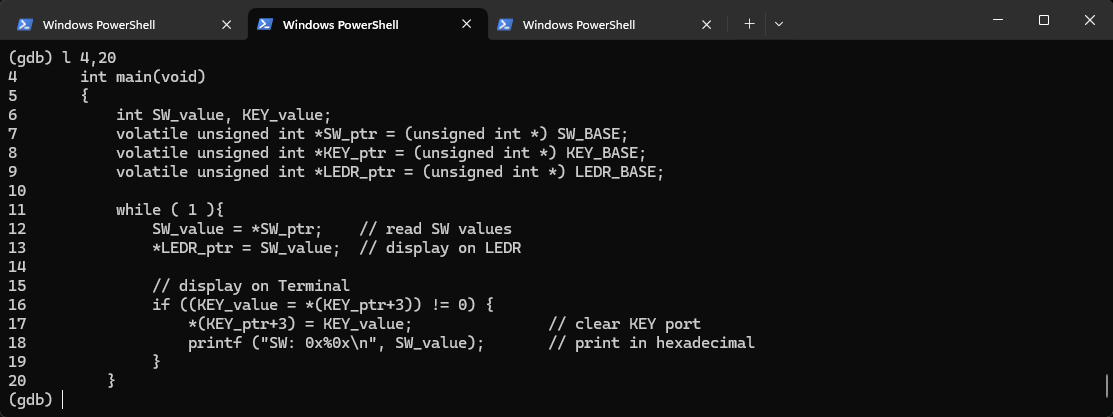
\includegraphics[scale=.6]{figures/print_C1.png}
        \caption{The {\it printf} example.}
        \label{fig:print_C1}
    \end{center}
\end{figure}

In the GDB Client, use \texttt{detach} to disconnect from the DE1-SoC board and then
\texttt{quit} from the GDB client. Also, quit from the GDB Server in its terminal window.
Finally, close the {\it nios2-terminal} by typing $^{\wedge}\texttt{C}$ in its window.

\newpage
\section*{Appendix A: GDB Command Reference}

Examples of GDB commands are summarized below. You can often execute a command by typing
only part of its name: for example {\bf s} executes the {\it step} command, {\bf b} executes
{\it break}, and {\bf cont} executes {\it continue}.

\begin{tabbing}
{\bf info address} symbol ~~~~\= ~~~~\=set a breakpoint at Line k in source code\kill
{\bf step} \>execute a single source-code line\\
{\bf step} {\it n} \>execute $n$ source-code lines\\
{\bf stepi} \>execute a single Nios~V machine instruction (not used in the tutorial)\\
{\bf continue} \>run the program from its current location\\
{\bf next} \>execute the next source-code line, stepping over a subroutine call\\
{\bf break} {\it k} \>set a breakpoint at Line k in source code\\
{\bf clear} {\it k} \>clear the breakpoint at Line k \\
{\bf info reg} [{\it name}, $\ldots$] \>show the current value of Nios~V register(s) {\it
name}, $\ldots$\\
{\bf info symbol} address \>give the address of a symbol\\
{\bf info address} symbol \>give the symbol at an address\\
{\bf info break} \>list all active breakpoints\\
{\bf set} \$name = {\it value} \>Set the contents of Nios~V register {\it name} to {\it value}\\
{\bf set} name = {\it value} \>Set the contents of {\it name} (for example, a variable) to {\it value}\\
{\bf delete} \>clear all active breakpoints\\
{\bf x} {\it A} \>display the word in memory at address {\it A}\\
{\bf x}/x {\it A} \>display the word in memory in hexadecimal at address {\it A}\\
{\bf x}/4x {\it A} \>display the four words in memory in hexadecimal starting at address {\it A}\\
{\bf x}/xb {\it A} \>display the byte in memory in hexadecimal at address {\it A}\\
{\bf print} {\it expr} \>print the value of an expression (for example, a variable)\\
{\bf print} /x {\it expr} \>print the value of an expression in hexadecimal\\
{\bf detach} \>disconnect the GDB Client from the target\\
{\bf quit} \>close the GDB client, or GDB Server\\
{\bf load} \>load the executable program into memory (used in Makefiles)\\
{\bf target remote} {\it port} \>connect to remote debugging {\it port} (used in Makefiles)
\end{tabbing}

% Copyright and Trademark

%\newcommand{\datePublished}{Mar 2022}

\newcommand{\versnum}{21.1} %version number quartus/AMP
\newcommand{\quartusname}{Quartus\textsuperscript{\textregistered} Prime}	
\newcommand{\textBar}{For \quartusname{} \versnum{}}
\newcommand{\thisyear}{2022 } %for copyright
\newcommand{\company}{FPGAcademy.org}
\newcommand{\longteamname}{FPGAcademy.org}
\newcommand{\teamname}{FPGAcademy}
\newcommand{\website}{FPGAcademy.org}

\newcommand{\productAcronym}{AMP}
\newcommand{\productNameShort}{Monitor Program}

\newcommand{\productNameMedTM}{Monitor Program}
\newcommand{\productNameMed}{Monitor Program}

%\newcommand{\headerLogoFilePath}[1]{#1/FPGAcademy.png}



%%%%%%%%%%%%%%%%%%%%%%%%%%%%%%%%%%%%%%%%
%%% FPGAcademy Copyright Information %%%
%%%%%%%%%%%%%%%%%%%%%%%%%%%%%%%%%%%%%%%%

%Always put the copyright on a new page (clear page), with some vertical space from top
\clearpage
\vspace{1in}

\noindent

Copyright {\copyright} FPGAcademy.org. All rights reserved. FPGAcademy and the FPGAcademy logo are trademarks of  FPGAcademy.org.  This document is being provided on an ``as-is'' basis and as an accommodation and therefore all warranties, representations or guarantees of any kind (whether express, implied or statutory) including, without limitation, warranties of merchantability, non-infringement, or fitness for a particular purpose, are specifically disclaimed.

%FPGAcademy assumes no responsibility or liability arising out of the application or use of any information,  product,  or  service  described  herein  except  as  expressly  agreed  to  in  writing  by  FPGAcademy.



**Other names and brands may be claimed as the property of others.




\end{document}
